\documentclass{SGGW-thesis}

\MAGISTERSKAtrue
\WZIMtrue

\title{Porównanie metod sekwencyjnych i grafowych\\w predykcji wiązania TCR-pMHC\\na przykładzie epitopu IE-1 wirusa CMV}
\Etitle{Comparison of Sequential and Graph-Based Methods\\for TCR-pMHC Binding Prediction:\\A Case Study on the IE-1 CMV Epitope}
\author{Ludwik Tarnicki}
\date{2026}
\album{s211052}
\thesis{Praca dyplomowa magisterska na kierunku:}
\course{Informatyka}
\promotor{dra hab.\ Bartosza Świderskiego}
\pworkplace{Katedra Sztucznej Inteligencji}

\usepackage{hyperref}
\usepackage{amsmath}
\usepackage{amssymb}
\usepackage{booktabs}
\usepackage{graphicx}
\usepackage{multirow}
\usepackage{array}
\usepackage{xcolor}
\usepackage{algorithm}
\usepackage{algpseudocode}
\usepackage[stretch=10,shrink=10]{microtype}

\widowpenalty=10000
\clubpenalty=10000

\renewcommand{\bibname}{Bibliografia}

\renewcommand{\abstractpage}[6]{%
    \setstretch{1.4}
    \null
    \vfill
    \begin{center}
        \textbf{Streszczenie}\\
    \end{center}
    \noindent
    \textbf{#1}\\[1.5ex]
    {#2}
    \\[4ex]
    Słowa kluczowe -- {#3}
    \ifthenelse{\equal{#4}{}}{}{%
        \vfill
        \begin{center}
            \textbf{Summary}\\
        \end{center}
        \noindent
        \textbf{#4}\\[1.5ex]
        {\selecthyphenation{english}#5}
        \\[4ex]
        Keywords -- {\selecthyphenation{english}#6}
    }%
    \vfill
    \pagestyle{empty}
    \newpage
    \null
    \pagestyle{empty}
    \newpage
    \pagestyle{plain}
}

\begin{document}
\maketitle
\statementpage
\abstractpage
{Porównanie metod sekwencyjnych i grafowych w predykcji wiązania TCR-pMHC na przykładzie epitopu IE-1 wirusa CMV}
{Niniejsza praca poświęcona jest problemowi predykcji wiązania receptora komórek T (TCR) z kompleksem
peptyd-MHC (pMHC) na przykładzie dominującego epitopu IE-1 wirusa cytomegalii (CMV). Zadanie to
posiada istotne znaczenie kliniczne: zrozumienie specyficzności TCR jest kluczowe dla projektowania
immunoterapii opartych na adoptywnym transferze limfocytów T. Ze względu na ogromną przestrzeń sekwencji
TCR oraz silne niezrównoważenie danych eksperymentalnych (stosunek pozytywów do negatywów wynosi
${\approx}1{:}8{,}6$ w~zbiorze roboczym, a~${\approx}1{:}18$ w~pełnym zbiorze IE-1 przed wykluczeniem
allelu pozbawionego sygnału pozytywnego), problem stanowi poważne wyzwanie obliczeniowe i statystyczne. W~pracy porównano cztery podejścia
modelowania: klasyfikator k najbliższych sąsiadów (k-NN) oparty na embeddingach ESM2, wielowarstwowy
perceptron (MLP), splotową sieć neuronową inspirowaną modelem NetTCR-2.0 oraz grafową sieć neuronową
(GNN) operującą na podgrafach k-NN sąsiedztwa biologicznego. Dla każdego modelu opisano architekturę,
zastosowane wzory matematyczne oraz procedurę treningu. Główną metryką oceny jest pole pod krzywą
precyzja-czułość (PR-AUC) wyznaczone metodą bootstrap z 95\% przedziałami ufności. Praca zawiera
szczegółowy opis \textit{pipeline'u} danych (od surowych obserwacji z~bazy TRAIT do podgrafów na potrzeby GNN). Wykazano przy tym, że wysokie wartości metryk agregatowych
w~znacznej mierze wynikają z~obecności w~zbiorze allelu HLA-A*24:02, który w~danych IE-1\_CMV
jest reprezentowany niemal wyłącznie przez obserwacje negatywne, a~rzeczywista zdolność
rozróżniania TCR w~obrębie allelu prezentującego jest istotna
statystycznie, lecz umiarkowana.}
{TCR-pMHC, CMV, predykcja wiązania TCR, grafowa sieć neuronowa, ESM2, NetTCR, klasyfikacja binarna, PR-AUC, immunoinformatyka}
{}
{}
{}

\tableofcontents

\startchapterfromoddpage

% ============================================================
\chapter{Wstęp}
\label{chap:wstep}
% ============================================================

\section{Kontekst kliniczny i motywacja}

Cytomegalowirus (CMV, ang.\ \textit{cytomegalovirus}) jest powszechnym, latentnym herpewirusem, który
infekuje od 60 do 90\% populacji światowej~\cite{sylwester2005}. U osób z prawidłową odpornością
zakażenie przebiega zazwyczaj bezobjawowo, jednak u~pacjentów immunosupresowanych (po przeszczepieniu
narządów lub szpiku kostnego, a~także u~osób zakażonych wirusem HIV) reaktywacja CMV może prowadzić
do poważnych powikłań klinicznych: zapalenia płuc, zapalenia siatkówki, zapalenia mózgu, a w skrajnych
przypadkach do zgonu~\cite{wills1996}. Kluczową rolę w~kontrolowaniu latencji wirusa odgrywają
cytotoksyczne limfocyty T~CD8$^+$ (CTL), które rozpoznają wirusowe peptydy prezentowane na cząsteczkach
MHC klasy~I na powierzchni zakażonych komórek.

Spośród licznych białek CMV szczególne znaczenie kliniczne ma antygen bezpośrednio wczesny IE-1
(ang.\ \textit{immediate-early 1}), który jest jednym z~pierwszych produktów ekspresji genu po
reaktywacji wirusa. Epitop pochodzący z~IE-1 i~prezentowany przez allel HLA-A*03:01 stanowi jeden
z~immunodominujących celów odpowiedzi CTL u~osób seropozytywnych~\cite{wills1996,sylwester2005}.
Sylwester i wsp.~\cite{sylwester2005} wykazali, że odpowiedź immunologiczna przeciwko CMV angażuje
od 4 do 10\% całkowitej puli cytotoksycznych limfocytów T~u~zdrowych dawców. Możliwość przewidywania,
które receptory TCR będą reagować na epitop IE-1, ma bezpośrednie implikacje dla adoptywnej terapii
komórkami T~- metody, w~której ex vivo namnażane limfocyty T~o~pożądanej specyficzności przenoszone
są do pacjenta w~celu eliminacji zakażonych komórek.

Predykcja specyficzności TCR jest jednak zadaniem wyjątkowo trudnym. Po pierwsze, przestrzeń możliwych
sekwencji TCR jest astronomiczna: repertuar TCR człowieka zawiera szacunkowo od $10^{15}$ do $10^{20}$
unikatowych klonotypów~\cite{moris2021}. Po drugie, dane eksperymentalne dotyczące wiązania TCR-pMHC
są silnie niezrównoważone: liczba obserwacji negatywnych (brak wiązania) wielokrotnie przewyższa
liczbę pozytywnych. Po trzecie, zdolność do wiązania zależy od subtelnych cech sekwencji, przede
wszystkim zmiennych pętli CDR3 łańcuchów $\alpha$ i~$\beta$ TCR, których matematyczna reprezentacja
nastręcza trudności.

\section{Cel i zakres pracy}

Celem niniejszej pracy jest systematyczne porównanie czterech klas metod uczenia maszynowego do binarnej
predykcji wiązania TCR-pMHC:
\begin{enumerate}
  \item klasyfikator $k$~najbliższych sąsiadów (k-NN) oparty na embeddingach ESM2,
  \item wielowarstwowy perceptron (MLP) operujący na uśrednionych embeddingach sekwencji,
  \item splotowa sieć neuronowa (CNN) inspirowana architekturą NetTCR-2.0~\cite{montemurro2022},
  \item grafowa sieć neuronowa (GNN) operująca na podgrafach k-NN sąsiedztwa biologicznego.
\end{enumerate}

Praca skupia się wyłącznie na epitopie IE-1 wirusa CMV, co pozwala na głęboką analizę jednego,
dobrze zdefiniowanego zadania. Zbiór danych pochodzi z~bazy TRAIT~\cite{trait} i~obejmuje ponad 267~000
eksperymentalnych obserwacji dla \textit{sparowanych} łańcuchów $\alpha$ i~$\beta$ TCR, co stanowi
istotną przewagę nad większością publicznych zbiorów danych zawierających jedynie łańcuch $\beta$.

\section{Hipoteza badawcza}

\textbf{Hipoteza zerowa (H$_0$):} Modele oparte wyłącznie na sekwencji (MLP, CNN) osiągają
porównywalne wartości PR-AUC co modele grafowe (GNN) na zadaniu predykcji wiązania TCR do
epitopu IE-1 wirusa CMV, tzn.\ architektura GNN z~grafem k-NN sąsiedztwa w~przestrzeni
embeddingów ESM2 nie wnosi istotnej przewagi predykcyjnej nad prostszymi modelami sekwencyjnymi.

Niezależnie od kierunku wyniki eksperymentu mają wartość poznawczą. Utrzymanie H$_0$
wskazywałoby, że embeddingi ESM2 same w~sobie kodują wystarczająco bogate reprezentacje
biologicznego sąsiedztwa i~prostsze modele sekwencyjne są wystarczające dla tego zadania.
Odrzucenie H$_0$ potwierdzałoby natomiast, że lokalna topologia przestrzeni TCR niesie
informację niedostępną modelom operującym na izolowanych embeddingach. Należy przy tym wyraźnie
podkreślić, że nieodrzucenie H$_0$ nie jest dowodem na jej prawdziwość (brak statystycznego
dowodu na różnicę $\neq$ dowód na brak różnicy), a~ewentualne odrzucenie nie implikuje
automatycznie żadnego konkretnego mechanizmu wyjaśniającego przewagę grafu.

\section{Struktura pracy}

Praca zorganizowana jest następująco. Rozdział~\ref{chap:tlo} przedstawia tło teoretyczne niezbędne
do zrozumienia problemu: biologię układu TCR-pMHC, znaczenie kliniczne wirusa CMV i epitopu IE-1,
metody embeddingu sekwencji białkowych opartych na modelu ESM2 oraz teorię grafowych sieci
neuronowych. Rozdział~\ref{chap:dane} opisuje zbiór danych, procedurę filtracji, podział na podzbiory
oraz \textit{pipeline} generowania embeddingów. Rozdział~\ref{chap:metody} zawiera szczegółowy opis
wszystkich czterech modeli wraz z~wzorami matematycznymi, strategię ewaluacji, procedurę treningu
oraz tabele wynikowe. Rozdział~\ref{chap:zakonczenie}
stanowi zakończenie zawierające podsumowanie wyników, dyskusję, ograniczenia badania oraz kierunki
przyszłych prac.


% ============================================================
\chapter{Tło teoretyczne}
\label{chap:tlo}
% ============================================================

\section{Biologia układu TCR-pMHC}

\subsection{Receptor komórek T: budowa i funkcja}

Receptor komórek T (TCR, ang.\ \textit{T~cell receptor}) jest białkiem obecnym na powierzchni
limfocytów T, odpowiedzialnym za rozpoznanie kompleksu peptyd-MHC (pMHC)~\cite{janeway2017}.
Receptor zbudowany jest z~dwóch łańcuchów: $\alpha$ i~$\beta$, z~których każdy zawiera trzy
regiony hiperzmienne (CDR1, CDR2, CDR3). Spośród nich CDR3 wykazuje najwyższą zmienność sekwencji
i~bezpośrednio kontaktuje się z~prezentowanym peptydem~\cite{janeway2017}.
Sekwencja CDR3 obu łańcuchów jest kluczowym wyznacznikiem specyficzności TCR i~stanowi
główne źródło informacji dla modeli predykcji.

\subsection{Główny układ zgodności tkankowej (MHC klasy~I)}

Cząsteczki MHC klasy~I (u~człowieka zwane HLA, ang.\ \textit{human leukocyte antigen})
są białkami obecnymi na powierzchni komórek, które prezentują krótkie fragmenty białek
wewnątrzkomórkowych (peptydy) limfocytom T~\cite{janeway2017}. Każdy allel MHC
preferencyjnie wiąże peptydy o~określonym wzorcu sekwencji. W~niniejszej pracy uwzględnione
są dwa allele: HLA-A*03:01 (dominujące źródło sygnału pozytywnego dla epitopu IE-1~CMV)
i~HLA-A*24:02.

\subsection{Mechanizm prezentacji antygenu i rozpoznania przez TCR}

Białka wirusowe ulegają wewnątrzkomórkowej degradacji do krótkich peptydów, które są ładowane
na cząsteczki MHC i~prezentowane na powierzchni komórki. Limfocyt T~rozpoznaje kompleks pMHC
poprzez swój TCR~\cite{wills1996}. Zdolność do wiązania zależy od sekwencji peptydu, allelu MHC
oraz sekwencji CDR3 obu łańcuchów TCR~\cite{janeway2017}. Ta wieloczynnikowa zależność
sprawia, że predykcja wiązania TCR-pMHC jest trudnym problemem zarówno dla metod klasycznych,
jak i~głębokiego uczenia.

\section{Wirus CMV i epitop IE-1}

Cytomegalowirus ludzki (HCMV) po pierwotnym zakażeniu pozostaje w~organizmie w~stanie latencji
i~może reaktywować się w~warunkach obniżonej odporności~\cite{sylwester2005}.
Białko IE-1 jest jednym z~pierwszych produktów ekspresji po reaktywacji wirusa.
Przedmiotem analizy w~niniejszej pracy jest rozpoznawanie epitopów białka IE-1 wirusa CMV przez
limfocyty T, w~kontekście dwóch obecnych w~danych kompleksów peptyd-MHC: peptydu \texttt{KLGGALQAK}
prezentowanego przez allel HLA-A*03:01 oraz peptydu \texttt{AYAQKIFKI} prezentowanego przez allel
HLA-A*24:02. Oba peptydy stanowią immunodominujące cele odpowiedzi limfocytów T~u~osób
seropozytywnych~\cite{wills1996,sylwester2005}.

\section{Reprezentacja sekwencji białkowych: model ESM2}

\subsection{Modele językowe dla sekwencji białkowych}

Modele językowe dużej skali (LLM, ang.\ \textit{large language models}), pierwotnie opracowane dla
języka naturalnego, z~powodzeniem zaadaptowano do modelowania sekwencji biologicznych, traktując
aminokwasy analogicznie do tokenów języka. Modele takie uczą się na dużych korpusach sekwencji
białkowych (setki milionów do miliardów sekwencji z~bazy UniRef) i~uchwytują ewolucyjne, strukturalne
i~funkcjonalne cechy białek w~sposób nienadzorowany~\cite{rives2021}.

Kluczową właściwością tych modeli jest zdolność do generowania kontekstowych embeddingów: reprezentacja
danego aminokwasu zależy nie tylko od niego samego, lecz od całej otaczającej sekwencji dzięki
mechanizmowi self-attention. Modele ESM~\cite{rives2021} i~ich następnik ESM2~\cite{lin2023}
zrewolucjonizowały dziedzinę bioinformatyki strukturalnej i~funkcjonalnej, umożliwiając predykcję
struktury białek na poziomie porównywalnym z~AlphaFold2.

\subsection{Architektura ESM2}

ESM2~\cite{lin2023} (\textit{Evolutionary Scale Modeling 2}) jest rodziną modeli białkowych opartych
na architekturze Transformer encoder-only, opracowaną przez Meta AI Research. W~niniejszej pracy
zastosowano model \texttt{esm2\_t30\_150M\_UR50D}, który zawiera 30~warstw transformerowych
i~generuje reprezentacje o~wymiarze $d = 640$. Model był trenowany na 250~milionach sekwencji
białkowych z~bazy UniRef50 metodą maskowanego modelowania języka (MLM, ang.\ \textit{masked language
modeling})~\cite{devlin2019}: 15\% aminokwasów w~sekwencji treningowej jest losowo maskowanych,
a~model uczy się przewidywać ich tożsamość na podstawie całego pozostałego kontekstu.

Formalnie, niech $\mathcal{M} \subset \{1, \ldots, L\}$ oznacza zbiór pozycji wybranych do
maskowania, a~$s_{\setminus \mathcal{M}}$~--- sekwencję z~zamaskowanymi tymi pozycjami. Model
minimalizuje skrośnoentropijną stratę przewidywania zamaskowanych aminokwasów:
\begin{equation}
    \mathcal{L}_{\mathrm{MLM}} = -\,\mathbb{E}_{s \sim \mathcal{D}}\,
    \mathbb{E}_{\mathcal{M}} \sum_{i \in \mathcal{M}} \log p_\theta\!\left(a_i \mid s_{\setminus \mathcal{M}}\right),
    \label{eq:mlm}
\end{equation}
gdzie $p_\theta(a_i \mid s_{\setminus \mathcal{M}})$ jest prawdopodobieństwem przypisanym przez model
prawdziwemu aminokwasowi $a_i$ na pozycji $i$, a~$\mathcal{D}$~--- rozkładem sekwencji treningowych
(UniRef50). Cel ten zmusza model do nauczenia się statystycznych zależności między pozycjami
w~sekwencji: aby trafnie odtworzyć zamaskowany aminokwas, sieć musi uchwycić ograniczenia
ewolucyjne, koewolucję reszt w~kontakcie przestrzennym oraz motywy funkcjonalne. To właśnie te
zależności, zakodowane implicytnie w~wagach modelu, sprawiają, że embeddingi ESM2 niosą informację
biologiczną użyteczną w~zadaniach pochodnych~--- takich jak predykcja wiązania TCR--pMHC~--- bez
konieczności jawnego nadzoru strukturalnego.

Dla sekwencji białkowej $s = (a_1, a_2, \ldots, a_L)$ o~długości $L$, model ESM2 produkuje macierz
reprezentacji per-residue:
\begin{equation}
    \mathbf{E} = \text{ESM2}(s) \in \mathbb{R}^{L \times d}, \qquad d = 640
    \label{eq:esm2_output}
\end{equation}
gdzie $\mathbf{E}_i \in \mathbb{R}^{640}$ jest embeddingiem $i$-tego aminokwasu z~uwzględnieniem
pełnego kontekstu sekwencji.

\subsubsection*{Architektura warstwy transformerowej}

Każda z~30 warstw enkodera ESM2 realizuje dwa bloki obliczeniowe: wielogłowy mechanizm
self-attention oraz sieć Feed-Forward (FFN), oba wyposażone w~połączenia rezydualne
i~normalizację warstwy (LayerNorm).

Niech $\mathbf{H}^{(l)} \in \mathbb{R}^{L \times d}$ oznacza macierz reprezentacji sekwencji
na wejściu $l$-tej warstwy. Dla każdej z~$H_{\text{heads}} = 20$ głowic uwagi wyznaczane są
trzy projekcje liniowe~\cite{vaswani2017}:
\begin{equation}
    \mathbf{Q}_h = \mathbf{H}^{(l)}\mathbf{W}_h^Q,\quad
    \mathbf{K}_h = \mathbf{H}^{(l)}\mathbf{W}_h^K,\quad
    \mathbf{V}_h = \mathbf{H}^{(l)}\mathbf{W}_h^V,
    \qquad \mathbf{W}_h^Q,\mathbf{W}_h^K,\mathbf{W}_h^V \in \mathbb{R}^{d \times d_k}
    \label{eq:qkv}
\end{equation}
gdzie $d_k = d / H_{\text{heads}} = 32$ jest wymiarem klucza na głowicę. Uwaga dla pojedynczej
głowicy obliczana jest przez skalowany iloczyn skalarny:
\begin{equation}
    \mathrm{Attention}(\mathbf{Q}_h, \mathbf{K}_h, \mathbf{V}_h)
    = \mathrm{softmax}\!\left(\frac{\mathbf{Q}_h \mathbf{K}_h^T}{\sqrt{d_k}}\right)\mathbf{V}_h
    \in \mathbb{R}^{L \times d_k}
    \label{eq:attention}
\end{equation}
Skalowanie przez $\sqrt{d_k}$ zapobiega zanikaniu gradientów w~rozkładzie softmax dla dużych
wartości iloczynu skalarnego. Wyjścia wszystkich głowic łączone są przez konkatenację
i~projekcję wyjściową:
\begin{equation}
    \mathrm{MHA}(\mathbf{H}) = \bigl[\mathrm{head}_1;\; \ldots;\; \mathrm{head}_{H_{\text{heads}}}\bigr]\mathbf{W}^O,
    \quad \mathrm{head}_h = \mathrm{Attention}(\mathbf{Q}_h, \mathbf{K}_h, \mathbf{V}_h),
    \quad \mathbf{W}^O \in \mathbb{R}^{d \times d}
    \label{eq:mha}
\end{equation}
Połączenia rezydualne i~normalizacja warstwy stabilizują trening~\cite{ba2016,vaswani2017}:
\begin{align}
    \mathbf{H}' &= \mathrm{LayerNorm}\!\left(\mathbf{H}^{(l)} + \mathrm{MHA}(\mathbf{H}^{(l)})\right)
    \label{eq:residual1} \\
    \mathbf{H}^{(l+1)} &= \mathrm{LayerNorm}\!\left(\mathbf{H}' + \mathrm{FFN}(\mathbf{H}')\right)
    \label{eq:residual2}
\end{align}
gdzie normalizacja warstwy dla wektora $\mathbf{h} \in \mathbb{R}^d$:
\begin{equation}
    \mathrm{LayerNorm}(\mathbf{h}) = \boldsymbol{\gamma} \odot
    \frac{\mathbf{h} - \mu_{\mathbf{h}}}{\sigma_{\mathbf{h}} + \epsilon} + \boldsymbol{\beta},
    \qquad \mu_{\mathbf{h}} = \tfrac{1}{d}\sum_j h_j,\quad
    \sigma_{\mathbf{h}} = \sqrt{\tfrac{1}{d}\sum_j (h_j - \mu_{\mathbf{h}})^2}
    \label{eq:layernorm}
\end{equation}
a~sieć FFN przekształca każdą pozycję niezależnie przez dwuwarstwową sieć z~aktywacją GELU:
\begin{equation}
    \mathrm{FFN}(\mathbf{h}) = \mathbf{W}_2\,\mathrm{GELU}(\mathbf{W}_1 \mathbf{h} + \mathbf{b}_1) + \mathbf{b}_2,
    \qquad \mathbf{W}_1 \in \mathbb{R}^{4d \times d},\; \mathbf{W}_2 \in \mathbb{R}^{d \times 4d}
    \label{eq:ffn}
\end{equation}

\subsubsection*{Kluczowe właściwości ESM2 istotne dla predykcji TCR}

Mechanizm self-attention umożliwia każdemu aminokwasowi $i$ agregowanie informacji ze
\textit{wszystkich} pozostałych pozycji $j$ sekwencji w~jednym kroku, bez ograniczeń
odległościowych charakterystycznych dla CNN ($\mathcal{O}(L)$ vs.\ $\mathcal{O}(1)$ skoków
informacji). Jest to szczególnie istotne dla pętli CDR3, gdzie kontakty z~peptydem zależą od
subtelnych, nielokalnych wzorców sekwencji. ESM2 stosuje ponadto obrotowe embeddingi pozycyjne
(RoPE, ang.\ \textit{Rotary Position Embeddings})~\cite{lin2023}, które kodują odległości względne między
pozycjami, co zapewnia lepszą generalizację na sekwencje o~długościach niespotykanych w~treningu.
Po 30 warstwach transformerowych zwrócona macierz $\mathbf{E}^{(30)} = \mathbf{H}^{(30)}$
stanowi wejście do dalszych modeli zgodnie z~równaniem~\eqref{eq:esm2_output}.

\subsection{Sposoby wykorzystania embeddingów ESM2}
\label{sec:esm2_usage}

W~niniejszej pracy stosowane są dwa warianty agregacji embeddingów:

\paragraph{Uśredniony embedding (mean-pooled).}
Reprezentacja całego łańcucha jako średnia po pozycjach:
\begin{equation}
    \bar{\mathbf{e}} = \frac{1}{L} \sum_{i=1}^{L} \mathbf{E}_i \in \mathbb{R}^{640}
    \label{eq:mean_pool}
\end{equation}
Stosowany w~modelach MLP i~GNN. Dla sparowanego TCR ($\alpha$ i~$\beta$) embeddingi obu łańcuchów
konkatenuje się w~wektor:
\begin{equation}
    \mathbf{z}_{\text{TCR}} = \left[\bar{\mathbf{e}}_\alpha;\; \bar{\mathbf{e}}_\beta\right] \in \mathbb{R}^{1280}
    \label{eq:tcr_concat}
\end{equation}

\paragraph{Embeddingi per-residue.}
Pełna macierz $\mathbf{E} \in \mathbb{R}^{L \times 640}$, zachowująca informację o~lokalizacji każdego
aminokwasu. Stosowana w~modelu CNN, który przetwarza sekwencję jako sygnał jednorodny o~zmiennej długości.

\subsection{Kodowanie allelu MHC}
\label{sec:mhc_encoding}

W~modelach MLP i~GNN dwa allele MHC obecne w~zbiorach uczących kodowane są jako wektor one-hot
$\mathbf{m} \in \{0,1\}^2$: HLA-A*03:01 reprezentowany jest przez $[1,\,0]$,
a~HLA-A*24:02 przez $[0,\,1]$. Kodowanie zachowuje pełną informację o~przynależności do allelu
przy minimalnej liczbie parametrów. Model CNN stosuje zamiast tego uczone osadzenie allelu
(\texttt{nn.Embedding}) w~przestrzeni $\mathbb{R}^{16}$, natomiast klasyfikator k-NN~---
równoważną binarną flagę allelu.

\section{Grafowe sieci neuronowe}

\subsection{Motywacja do użycia GNN}

Strukturę danych TCR można ująć w~naturalny sposób jako graf: węzły reprezentują poszczególne TCR,
a~krawędzie (mierzone podobieństwem kosinusowym embeddingów ESM2) kodują biologiczne sąsiedztwo
w~przestrzeni sekwencji. Hipoteza stojąca za modelem GNN jest następująca: TCR podobne sekwencyjnie
(i~embeddingowo) wykazują podobny profil wiązania, a~zatem agregacja informacji od sąsiadów w~grafie
powinna poprawić predykcję dla konkretnego TCR docelowego.

\subsection{Splotowe sieci grafowe (GCN)}

Graf $G = (V, E)$ definiuje się przez zbiór węzłów $V$, zbiór krawędzi $E \subseteq V \times V$
i~macierz sąsiedztwa $\mathbf{A} \in \mathbb{R}^{|V| \times |V|}$ (ewentualnie ważoną). Każdy
węzeł $v \in V$ ma przypisany wektor cech $\mathbf{x}_v \in \mathbb{R}^d$.

Kipf i~Welling~\cite{kipf2017} zaproponowali warstwę GCN (\textit{Graph Convolutional Network}),
w~której reguła propagacji dla $l$-tej warstwy wynosi:
\begin{equation}
    \mathbf{H}^{(l+1)} = \sigma\!\left(\tilde{\mathbf{D}}^{-1/2}\tilde{\mathbf{A}}\tilde{\mathbf{D}}^{-1/2}\mathbf{H}^{(l)}\mathbf{W}^{(l)}\right)
    \label{eq:gcn}
\end{equation}
gdzie $\tilde{\mathbf{A}} = \mathbf{A} + \mathbf{I}$ jest macierzą sąsiedztwa z~pętelkami własnymi,
$\tilde{\mathbf{D}}_{ii} = \sum_j \tilde{\mathbf{A}}_{ij}$ jest macierzą stopni,
$\mathbf{W}^{(l)} \in \mathbb{R}^{d_l \times d_{l+1}}$ jest uczalną macierzą wag warstwy $l$,
a~$\sigma$ jest nieliniową funkcją aktywacji. Człon $\tilde{\mathbf{D}}^{-1/2}\tilde{\mathbf{A}}\tilde{\mathbf{D}}^{-1/2}$
stanowi symetrycznie znormalizowaną macierz sąsiedztwa, zapobiegającą skalowaniu reprezentacji
proporcjonalnie do stopnia węzła.

Równanie~\eqref{eq:gcn} można zinterpretować jako uśrednienie (z~wagami proporcjonalnymi do
znormalizowanego stopnia) cech sąsiadów węzła, a~następnie przekształcenie liniowe z~nieliniowością.
Warstwa GCN jest specjalnym przypadkiem zasady przekazywania wiadomości (\textit{message passing})~\cite{kipf2017}.

\subsection{GraphSAGE i sieci z mechanizmem uwagi: przegląd alternatyw}

Hamilton i~wsp.~\cite{hamilton2017} zaproponowali indukcyjny wariant GNN nazwany GraphSAGE
(\textit{SAmple and aggreGatE}), który zamiast używać pełnej macierzy sąsiedztwa próbkuje
podzbiór sąsiadów każdego węzła. Reguła agregacji (wariant uśredniający) dla węzła $v$:
\begin{equation}
    \mathbf{h}_v^{(l+1)} = \sigma\!\left(\mathbf{W}^{(l)} \cdot \left[\mathbf{h}_v^{(l)};\;
    \frac{1}{|\mathcal{N}(v)|}\sum_{u \in \mathcal{N}(v)} \mathbf{h}_u^{(l)}\right]\right)
    \label{eq:graphsage}
\end{equation}
gdzie $[\cdot;\cdot]$ oznacza konkatenację, a~$\mathcal{N}(v)$ jest próbkowanym podzbiorem sąsiadów $v$.
Indukcyjność GraphSAGE pozwala na generalizację do węzłów nieobecnych podczas treningu,
co czyni go atrakcyjnym w~scenariuszach dużych, dynamicznych grafów.

Veličković i~wsp.~\cite{velickovic2018} zaproponowali \textit{Graph Attention Networks} (GAT),
w~których waga krawędzi $(v, u)$ wyznaczana jest przez uczony mechanizm uwagi:
\begin{equation}
    \alpha_{vu} = \frac{\exp\!\left(\mathrm{LeakyReLU}\!\left(\mathbf{a}^T\left[\mathbf{W}\mathbf{h}_v \,\|\, \mathbf{W}\mathbf{h}_u\right]\right)\right)}
    {\displaystyle\sum_{k \in \mathcal{N}(v)} \exp\!\left(\mathrm{LeakyReLU}\!\left(\mathbf{a}^T\left[\mathbf{W}\mathbf{h}_v \,\|\, \mathbf{W}\mathbf{h}_k\right]\right)\right)},
    \qquad \mathbf{h}_v^{(l+1)} = \sigma\!\left(\sum_{u \in \mathcal{N}(v)} \alpha_{vu}\,\mathbf{W}\mathbf{h}_u^{(l)}\right)
    \label{eq:gat}
\end{equation}
gdzie $\mathbf{a} \in \mathbb{R}^{2d'}$ i~$\mathbf{W} \in \mathbb{R}^{d' \times d}$ są uczonymi parametrami.
Wagi $\alpha_{vu}$ umożliwiają modelowi skupienie się na najbardziej informatywnych sąsiadach.

\subsection{Uzasadnienie wyboru warstwy GCNConv}
\label{sec:gcn_choice}

Spośród dostępnych architektur grafowych w~niniejszej pracy wybrano warstwę GCNConv~\cite{kipf2017}
z~trzech wzajemnie uzupełniających się powodów.

\textbf{Małe, gęste podgrafy.} Podgrafy konstruowane dla GNN mają 100--200 węzłów. GraphSAGE
jest zaprojektowany dla dużych grafów, w~których pełne przejście po sąsiedztwie jest
obliczeniowo prohibicyjne; przy tak małych grafach próbkowanie wprowadza niepotrzebną
wariancję. GCN korzysta z~pełnej macierzy sąsiedztwa, co jest dokładniejsze i~tańsze.

\textbf{Sensowne, prekomputowane wagi krawędzi.} Krawędziom przypisane są wagi oparte na
podobieństwie kosinusowym embeddingów ESM2 (wzór~\eqref{eq:edge_weight}), biologicznie
uzasadniona miara bliskości sekwencyjnej. GAT nadpisywałby te wagi uczonymi współczynnikami
uwagi, wprowadzając dodatkowe parametry i~ryzyko nadmiernego dopasowania przy ograniczonej
liczbie pozytywnych próbek treningowych ($\sim$14~000). GCN wbudowuje prekomputowane wagi
bezpośrednio w~znormalizowaną macierz sąsiedztwa $\tilde{\mathbf{D}}^{-1/2}\tilde{\mathbf{A}}\tilde{\mathbf{D}}^{-1/2}$.

\textbf{Prostota i~stabilność.} Warstwa GCN ma mniej parametrów niż GAT (brak uczonych wag
uwagi) i~zapewnia spektralnie uzasadnioną, symetryczną agregację sąsiedztwa. Połączona z~sieciami
JK~\cite{xu2018} (sekcja~\ref{sec:jk}) i~połączeniami rezydualnymi (wzór~\eqref{eq:gnn_gcn})
daje wieloskokową agregację z~kontrolowanym wygładzaniem, co jest wystarczające dla zadania
predykcji w~małych podgrafach biologicznych.

\subsection{Jumping Knowledge Networks}
\label{sec:jk}

Xu i~wsp.~\cite{xu2018} zaobserwowali, że w~głębokich GNN informacja z~odległych węzłów może dominować
nad lokalną strukturą wskutek nadmiernego wygładzania (\textit{over-smoothing})~\cite{oono2020}.

Zjawisko to ma ścisłe ujęcie teoretyczne. Operator propagacji GCN, $\hat{\mathbf{A}} =
\tilde{\mathbf{D}}^{-1/2}\tilde{\mathbf{A}}\tilde{\mathbf{D}}^{-1/2}$, jest macierzą o~wartościach
własnych w~przedziale $(-1, 1]$, przy czym największa wartość własna równa $1$ odpowiada wektorowi
własnemu związanemu ze~stopniami węzłów. Wielokrotne zastosowanie $\hat{\mathbf{A}}$ (czyli stos
$L$~warstw GCN) działa jak filtr dolnoprzepustowy na grafie: składowe odpowiadające mniejszym
wartościom własnym są tłumione wykładniczo z~głębokością. W~granicy $L \to \infty$ reprezentacje
węzłów w~obrębie spójnej składowej zbiegają do wspólnego, proporcjonalnego do stopnia wektora,
tracąc zdolność rozróżniania węzłów~\cite{oono2020}. Formalnie, odległość reprezentacji od tej
zdegenerowanej podprzestrzeni maleje jak $\mathcal{O}(\lambda^L)$, gdzie $\lambda < 1$ jest drugą
co do wielkości (co do modułu) wartością własną $\hat{\mathbf{A}}$.

Konsekwencja praktyczna jest istotna dla niniejszej pracy: w~zadaniu, w~którym najbardziej
informacyjny jest sam węzeł docelowy oraz jego najbliższe otoczenie, zwiększanie głębokości sieci
może \textit{szkodzić}. Wynik ablacji (rozdział~\ref{chap:metody}, tabela~\ref{tab:ablation_gnn}),
w~którym najpłytszy wariant $L{=}1$ osiąga najwyższą wartość PR-AUC, jest spójny z~tą interpretacją:
przy zadanej topologii ego-podgrafu agregacja z~odległości większej niż jeden skok nie wnosi
użytecznej informacji, a~głębsze warianty zaczynają podlegać wygładzaniu.

Aby częściowo przeciwdziałać temu zjawisku, zastosowano schemat \textit{Jumping Knowledge} (JK),
w~którym końcowa reprezentacja węzła $v$ jest agregacją reprezentacji ze \textit{wszystkich} warstw:
\begin{equation}
    \mathbf{h}_v^{\mathrm{JK}} = \mathrm{AGG}\!\left(\mathbf{h}_v^{(0)},\, \mathbf{h}_v^{(1)},\, \ldots,\, \mathbf{h}_v^{(L)}\right)
    \label{eq:jk}
\end{equation}
W~niniejszej pracy stosuje się agregację maksimum (max-pooling po warstwach), co pozwala modelowi
wybrać najbardziej informacyjną warstwę dla każdego wymiaru cech.

\section{Metody podgrafowe}

\subsection{SEAL i predykcja wiązań w grafach}

Zhang i~Chen~\cite{zhang2018seal} zaproponowali metodę SEAL (\textit{Subgraph Extraction and Labeling})
do predykcji wiązań w~grafach (\textit{link prediction}). Kluczowym spostrzeżeniem jest, że predykcja
wiązania między węzłami $(u, v)$ może być sformułowana jako klasyfikacja podgrafu: wyodrębnia się
ego-graf wokół pary $(u, v)$ i~klasyfikuje się go. Teru i~wsp.~\cite{teru2020} rozszerzyli tę ideę
na indukcyjne rozumowanie relacyjne w~modelu GraIL.

\subsection{Labeling Trick}

Aby umożliwić GNN rozróżnienie węzła docelowego od jego sąsiadów w~podgrafie, Zhang i~wsp.~\cite{zhang2021labeling}
formalnie uzasadnili zastosowanie etykiet pozycyjnych (\textit{labeling trick}). Każdy węzeł $v$
w~podgrafie wokół węzła docelowego $T^*$ otrzymuje dodatkową cechę kodującą jego odległość od $T^*$.

Bez takiej etykiety GNN nie może odróżnić węzła docelowego od jego sąsiadów, co prowadzi do
niezdolności do reprezentowania konkretnych węzłów w~podgrafie. W~niniejszej pracy etykiety pozycyjne
implementowane są jako czteroelementowy wektor \textit{one-hot} $\boldsymbol{\ell}_v \in \{0,1\}^4$,
gdzie kolejne bity odpowiadają: $(v = T^*)$, $d(v, T^*) = 1$, $d(v, T^*) = 2$, $d(v, T^*) \geq 3$,
a~$d$ oznacza odległość BFS w~grafie sąsiedztwa.


% ============================================================
\chapter{Przegląd literatury: metody predykcji TCR--pMHC}
\label{chap:przeglad}
% ============================================================

Problem komputerowej predykcji wiązania TCR--pMHC doczekał się w~ostatnich latach licznych podejść,
różniących się reprezentacją wejścia, architekturą oraz zakładanym scenariuszem generalizacji.
Niniejszy rozdział systematyzuje najważniejsze z~nich i~pozycjonuje względem nich metody zbadane
w~tej pracy. Wspólnym mianownikiem pozostaje trudność wynikająca z~ogromnej różnorodności repertuaru
TCR oraz silnego niezrównoważenia danych eksperymentalnych~\cite{moris2021}.

\section{Metody oparte na podobieństwie sekwencji}

Najwcześniejsze podejścia opierały się na założeniu, że TCR o~podobnych sekwencjach CDR3 rozpoznają
ten sam epitop. \textbf{GLIPH}~\cite{glanville2017} grupuje receptory w~„specificity groups" na
podstawie wspólnych motywów CDR3$\beta$ oraz globalnego podobieństwa sekwencji, wykorzystując
wzbogacenie motywów względem tła repertuaru. Metody klastrujące tego typu są interpretowalne
i~nie wymagają treningu z~nadzorem, lecz słabo generalizują na epitopy reprezentowane przez
nieliczne przykłady i~nie wykorzystują informacji o~allelu MHC. Klasyfikator k-NN badany w~niniejszej
pracy (rozdział~\ref{chap:metody}) należy konceptualnie do tej rodziny~--- różnicą jest zastąpienie
ręcznie definiowanych miar podobieństwa sekwencji odległością kosinusową w~przestrzeni embeddingów
ESM2, co pozwala uchwycić podobieństwo semantyczne, a~nie tylko literalne.

\section{Modele splotowe i rekurencyjne}

Przełomem było zastosowanie splotowych sieci neuronowych operujących bezpośrednio na zakodowanych
sekwencjach. \textbf{NetTCR}~\cite{jurtz2018} jako jeden z~pierwszych modeli wykorzystał konwolucje
1D do predykcji wiązania TCR$\beta$--peptyd dla allelu HLA-A*02:01, kodując aminokwasy macierzami
BLOSUM. Jego rozwinięcie, \textbf{NetTCR-2.0}~\cite{montemurro2022}, wprowadziło wykorzystanie
\textit{sparowanych} łańcuchów $\alpha$ i~$\beta$, wykazując, że dostęp do obu łańcuchów istotnie
poprawia jakość predykcji~--- pod warunkiem dysponowania co najmniej ${\sim}150$~parami na epitop.
Model splotowy badany w~tej pracy (rozdział~\ref{chap:metody}) jest bezpośrednio inspirowany
architekturą NetTCR-2.0, lecz operuje na per-residue'owych embeddingach ESM2 zamiast kodowania
BLOSUM, co stanowi istotną różnicę w~reprezentacji wejścia.

\textbf{ERGO}~\cite{springer2020} porównał kodery oparte na LSTM oraz na autoenkoderze, trenując
model na dużych słownikach par TCR--peptyd z~baz VDJdb i~McPAS-TCR. Praca ta uwypukliła kluczowy
problem metodologiczny: jakość predykcji silnie zależy od sposobu doboru przykładów negatywnych
oraz od tego, czy epitopy testowe były widziane podczas treningu.

\section{Modele z~mechanizmem uwagi i~uczeniem transferowym}

Nowsza generacja modeli wykorzystuje mechanizm uwagi oraz reprezentacje wstępnie wytrenowane.
\textbf{TITAN}~\cite{weber2021} stosuje dwumodalne sieci uwagi, przetwarzając równolegle sekwencję
TCR oraz strukturę SMILES peptydu, co umożliwia częściową generalizację na niewidziane epitopy.
\textbf{pMTnet}~\cite{lu2021} łączy uczenie transferowe: koder pMHC wstępnie trenowany na danych
o~prezentacji antygenu zostaje połączony z~koderem TCR, dzięki czemu model lepiej radzi sobie
z~neoantygenami reprezentowanymi przez nieliczne dane. \textbf{DLpTCR}~\cite{xu2021dlptcr} jest
z~kolei frameworkiem zespołowym (\textit{ensemble}), łączącym kilka architektur głębokich
i~obsługującym zarówno pojedyncze, jak i~sparowane łańcuchy.

Reprezentacje z~białkowych modeli językowych, takich jak ESM2~\cite{rives2021,lin2023}, stanowią
naturalne rozwinięcie tego nurtu: zamiast trenować koder sekwencji od podstaw, wykorzystuje się
kontekstowe embeddingi nauczone na milionach sekwencji białkowych. Wszystkie cztery modele badane
w~niniejszej pracy korzystają z~tej samej przestrzeni embeddingów ESM2, co pozwala odizolować wpływ
\textit{architektury} klasyfikatora od wpływu \textit{reprezentacji} wejścia.

\section{Podejścia grafowe}

Zastosowanie grafowych sieci neuronowych do predykcji TCR--pMHC jest stosunkowo nowe. Motywacją jest
hipoteza, że lokalna struktura sąsiedztwa w~przestrzeni receptorów niesie informację o~wspólnej
specyficzności~--- analogicznie do założenia metod klastrujących typu GLIPH, lecz wyrażonego w~języku
propagacji komunikatów w~grafie. Niniejsza praca wpisuje się w~ten nurt, konstruując ego-podgrafy
k-NN w~przestrzeni ESM2 i~stosując warstwy GCNConv (rozdział~\ref{chap:metody}). Otwartym pytaniem,
które praca stawia wprost w~hipotezie badawczej, jest to, czy taka topologia grafu wnosi informację
nieobecną już w~samych embeddingach.

\begin{table}[htbp]
\centering
\small
\caption{Zestawienie wybranych metod predykcji TCR--pMHC. Kolumna „Łańcuchy" wskazuje, czy model
korzysta z~pojedynczego łańcucha $\beta$, czy ze~sparowanych $\alpha{+}\beta$.}
\label{tab:related_work}
\begin{tabular}{lllc}
\toprule
\textbf{Metoda} & \textbf{Reprezentacja / architektura} & \textbf{Łańcuchy} & \textbf{Rok} \\
\midrule
GLIPH~\cite{glanville2017}        & motywy CDR3 + klastrowanie        & $\beta$            & 2017 \\
NetTCR~\cite{jurtz2018}           & BLOSUM + CNN 1D                   & $\beta$            & 2018 \\
ERGO~\cite{springer2020}          & LSTM / autoenkoder                & $\beta$            & 2020 \\
NetTCR-2.0~\cite{montemurro2022}  & BLOSUM + CNN 1D                   & $\alpha{+}\beta$   & 2021 \\
TITAN~\cite{weber2021}            & dwumodalna uwaga (TCR + SMILES)   & $\beta$            & 2021 \\
pMTnet~\cite{lu2021}              & uczenie transferowe + uwaga       & $\beta$            & 2021 \\
DLpTCR~\cite{xu2021dlptcr}        & zespół sieci głębokich            & $\alpha{+}\beta$   & 2021 \\
\midrule
\textbf{Niniejsza praca}          & ESM2 + MLP/CNN/GNN                & $\alpha{+}\beta$   & 2026 \\
\bottomrule
\end{tabular}
\end{table}

\section{Wyzwanie generalizacji na niewidziane epitopy}

Krytyczny przegląd Morisa i~wsp.~\cite{moris2021} zwrócił uwagę, że większość publikowanych modeli
osiąga wysokie wyniki wyłącznie w~scenariuszu \textit{seen-epitope} (epitopy testowe obecne podczas
treningu), a~ich jakość drastycznie spada przy predykcji dla całkowicie nowych epitopów. Niniejsza
praca świadomie ogranicza się do pojedynczego, dobrze scharakteryzowanego epitopu IE-1, co pozwala
na pogłębioną analizę porównawczą architektur, lecz nie odpowiada na pytanie o~generalizację
\textit{zero-shot}~--- kwestię tę wskazano jako kierunek dalszych badań (sekcja~\ref{sec:limitations}).

% ============================================================
\chapter{Przygotowanie danych}
\label{chap:dane}
% ============================================================

\section{Zbiór danych TRAIT}

Dane eksperymentalne pochodzą z~bazy TRAIT~\cite{trait} (\textit{T-cell Receptor--Antigen Interactions}),
która agreguje wyniki badań aktywacji TCR uzyskane metodami opartymi
na sekwencjonowaniu jednokomórkowym. Istotną cechą bazy jest obecność \textit{sparowanych} sekwencji
łańcuchów $\alpha$ i~$\beta$ TCR. Stanowi to przewagę nad bazami VDJdb, IEDB czy McPAS-TCR,
które w~dużej mierze zawierają jedynie łańcuch $\beta$, dostarczając przez to niekompletnej
informacji o~specyficzności receptora.

Każda obserwacja w~zbiorze TRAIT zawiera:
\begin{itemize}
  \item sekwencję CDR3 łańcucha $\alpha$ i~segmenty genowe (V, J),
  \item sekwencję CDR3 łańcucha $\beta$ i~segmenty genowe (V, D, J),
  \item identyfikator allelu MHC,
  \item identyfikator peptydu (epitopu),
  \item etykietę binarną: $y = 1$ (wiązanie) lub $y = 0$ (brak wiązania).
\end{itemize}

\section{Filtracja do epitopu IE-1\_CMV}

Z~pełnego zbioru zawierającego ponad 3,9~miliona obserwacji obejmujących liczne epitopy i~allele
MHC wyodrębniono wyłącznie obserwacje spełniające warunek \texttt{Epitope = IE-1\_CMV}. Następnie
wykluczono allel HLA-A*01:01, dla którego baza zawiera wyłącznie obserwacje negatywne (brak sygnału
pozytywnego, a~zatem brak wartości dyskryminacyjnej dla zadania). Pozostałe obserwacje dotyczą
\textbf{dwóch alleli MHC} (HLA-A*03:01 oraz HLA-A*24:02). Kolejne etapy redukcji liczebności
zestawia tabela~\ref{tab:dataflow}; szczegółowy rozkład po allelach przedstawia
tabela~\ref{tab:dataset_stats}.

\begin{table}[htbp]
\centering
\small
\caption{Przepływ danych: liczebność obserwacji na kolejnych etapach filtracji oraz w~podzbiorach
uczących. Stosunek pozytywów do negatywów ulega istotnej zmianie po wykluczeniu allelu HLA-A*01:01
(samych negatywów): z~${\approx}1{:}18$ na zbiorze IE-1\_CMV do ${\approx}1{:}8{,}6$ po wykluczeniu.
Częstość klasy pozytywnej jest zachowana we~wszystkich trzech podzbiorach (${\approx}10{,}5\%$),
co potwierdza poprawność stratyfikacji podziału per-TCR.}
\label{tab:dataflow}
\begin{tabular}{lcccc}
\toprule
\textbf{Etap} & \textbf{Obserwacje} & \textbf{Pozytywy} & \textbf{Częstość poz.} & \textbf{pos:neg} \\
\midrule
TRAIT (wiele epitopów)        & ${\approx}3{,}9$\,mln & ---     & ---       & --- \\
Po filtracji do IE-1\_CMV     & ${\approx}267\,000$   & 13~906  & ${\approx}5{,}2\%$  & 1:18 \\
Po wykluczeniu HLA-A*01:01    & 133~914               & 13~906  & $10{,}4\%$ & 1:8,6 \\
\midrule
\quad Zbiór treningowy        & 85~588                & 8~806   & $10{,}3\%$ & 1:8,7 \\
\quad Zbiór walidacyjny       & 23~968                & 2~531   & $10{,}6\%$ & 1:8,5 \\
\quad Zbiór testowy           & 24~358                & 2~569   & $10{,}6\%$ & 1:8,5 \\
\bottomrule
\end{tabular}
\end{table}

\begin{table}[htbp]
\centering
\small
\caption{Statystyki zbioru danych po filtracji do epitopu IE-1\_CMV (allele uwzględnione w~zbiorach uczących).}
\label{tab:dataset_stats}
\begin{tabular}{lccc}
\toprule
\textbf{Allel MHC} & \textbf{Obserwacje łącznie} & \textbf{Pozytywne ($y{=}1$)} & \textbf{Stosunek pos:neg} \\
\midrule
HLA-A*03:01 & ${\approx}66\,957$ & ${\approx}13\,880$ & 1:4 \\
HLA-A*24:02 & ${\approx}66\,957$ & ${\approx}30$      & rzadki sygnał \\
\midrule
\textbf{Łącznie} & \textbf{133~914} & \textbf{13~906} & \textbf{1:8,6} \\
\bottomrule
\end{tabular}
\end{table}

Dominacja allelu HLA-A*03:01 w~kontekście obserwacji pozytywnych wynika z~tego, że w~zbiorze
IE-1\_CMV niemal wszystkie udokumentowane wiązania dotyczą kompleksu \texttt{KLGGALQAK}/HLA-A*03:01;
kompleks \texttt{AYAQKIFKI}/HLA-A*24:02 dostarcza jedynie ${\approx}30$~obserwacji pozytywnych
(rzadki sygnał). Globalny stosunek pozytywów do negatywów po wykluczeniu
allelu HLA-A*01:01 wynosi ${\approx}1{:}8{,}6$ (na pełnym zbiorze IE-1\_CMV, przed wykluczeniem,
było to ${\approx}1{:}18$), co i~tak stanowi poważne wyzwanie dla metod uczenia maszynowego.

\section{Podział na zbiory: strategia per-TCR}

\subsection{Motywacja}

Naiwny losowy podział obserwacji prowadziłby do \textit{wycieku danych} (ang.\ \textit{data leakage}):
ten sam TCR mógłby wystąpić zarówno w~zbiorze treningowym, jak i~testowym. Model poznałby wtedy
konkretne sekwencje TCR zamiast uczyć się ogólnych cech determinujących wiązanie z~pMHC.
Aby temu zapobiec, zastosowano podział per-TCR: \textit{wszystkie} obserwacje danego TCR trafiają
do jednego i~tego samego podzbioru.

\subsection{Procedura podziału}

\begin{enumerate}
  \item Wyznaczono listę unikatowych par (CDR3$_\alpha$, CDR3$_\beta$) w~zbiorze IE-1\_CMV
        (66~957 unikatowych klonotypów).
  \item Przyjęto docelowy podział ${\approx}60/20/20\%$ (trening/walidacja/test): jako próg dla
        zbioru testowego i~walidacyjnego ustalono po ${\approx}20\%$ ogólnej liczby obserwacji.
        Klonotypy losowano z~ustalonym ziarnem (\texttt{seed = 42}) partiami i~przydzielano kolejno
        do zbioru testowego, a~następnie walidacyjnego, aż do osiągnięcia progu liczby obserwacji;
        pozostałe klonotypy utworzyły zbiór treningowy. Ponieważ klonotypy różnią się liczbą
        powiązanych obserwacji, a~przydział następował partiami, zrealizowany podział nieznacznie
        odbiega od wartości docelowych i~wynosi ${\approx}64/18/18\%$ zarówno na poziomie
        unikatowych TCR (42~794 / 11~984 / 12~179), jak i~obserwacji
        (85~588 / 23~968 / 24~358; tabela~\ref{tab:dataflow}).
  \item Każdej obserwacji przypisano przynależność do podzbioru zgodnie z~jej TCR.
\end{enumerate}

\subsection{Walidacja podziału}

Poprawność podziału zweryfikowano, sprawdzając:
\begin{itemize}
  \item zerowe przecięcie zbiorów TCR (brak wspólnych klonotypów między podzbiorami),
  \item zachowanie proporcji pos:neg w~każdym podzbiorze (podobne niezrównoważenie),
  \item zbliżoną dystrybucję alleli MHC w~każdym podzbiorze.
\end{itemize}

\section{Pipeline embeddingów ESM2}

\subsection{Generowanie embeddingów sekwencji TCR}

Dla każdego unikatowego TCR ($\alpha$, $\beta$) generowane są embeddingi przy użyciu modelu
\texttt{esm2\_t30\_150M\_UR50D} załadowanego przez interfejs PyTorch~\cite{paszke2019} (\texttt{torch.hub}) z~repozytorium
\texttt{facebookresearch/esm}. Model przetwarza sekwencję aminokwasową łańcucha i~zwraca:
\begin{itemize}
  \item \textbf{Mean-pooled embedding} $\bar{\mathbf{e}} \in \mathbb{R}^{640}$ (wzór~\eqref{eq:mean_pool}),
        zapisywany dla modeli MLP i~GNN.
  \item \textbf{Embeddingi per-residue} $\mathbf{E} \in \mathbb{R}^{L \times 640}$, zapisywane
        dla modelu CNN.
\end{itemize}

Sparowane embeddingi mean-pooled konkatenuje się zgodnie z~wzorem~\eqref{eq:tcr_concat} do wektora
$\mathbf{z}_{\mathrm{TCR}} \in \mathbb{R}^{1280}$.

\subsection{Kodowanie allelu MHC}

Allele MHC kodowane są binarnie zgodnie z~opisem w~sekcji~\ref{sec:mhc_encoding}. Wynikowy wektor
$\mathbf{m} \in \{0,1\}^2$ jest konkatenowany z~embeddingiem TCR na wejściu modelu.

\subsection{Budowa indeksu k-NN dla GNN}

Na potrzeby efektywnego wyszukiwania sąsiadów budowany jest indeks k-NN na zbiorze
embeddingów $\mathbf{z}_{\mathrm{TCR}} \in \mathbb{R}^{1280}$ wszystkich TCR ze zbioru
treningowego. W~implementacji zastosowano bibliotekę scikit-learn~\cite{pedregosa2011}
(\texttt{NearestNeighbors} z~metryką kosinusową), co zapewnia deterministyczne
wyniki wyszukiwania $k$ najbliższych sąsiadów. Indeks jest zapisywany na dysku i~ładowany
przy budowaniu podgrafów on-the-fly podczas treningu GNN.

\subsection{Prekomputacja podgrafów walidacyjnych i testowych}

Podgrafy dla zbiorów walidacyjnego i~testowego budowane są jednorazowo przed treningiem (dla każdej
pary TCR-MHC w~tych zbiorach) i~zapisywane na dysku jako pliki \texttt{.pt}. Każdy plik zawiera:
macierz cech węzłów $\mathbf{X}$, listę krawędzi, wagi krawędzi, indeks węzła docelowego $T^*$
oraz etykietę $y$. Szczegółowy opis struktury podgrafu zawarty jest w~sekcji~\ref{sec:gnn_graph_construction}.


% ============================================================
\chapter{Materiały i metody}
\label{chap:metody}
% ============================================================

\section{Strategia ewaluacji}
\label{sec:evaluation}

\subsection{Krzywa precyzja-czułość i PR-AUC}

Silne niezrównoważenie klas ($N_+ / N \approx 0{,}105$) sprawia, że standardowe metryki jak
dokładność (\textit{accuracy}) i~ROC-AUC są mylące: wysoka wartość ROC-AUC może wynikać z~dobrej
klasyfikacji klasy majorytarnej (negatywów), nie zaś z~wykrywania prawdziwych pozytywów~\cite{davis2006}.
W~niniejszej pracy główną metryką jest \textbf{PR-AUC} (pole pod krzywą precyzja-czułość).

Precyzja i~czułość (pełność, ang.\ \textit{recall}) definiowane są jako~\cite{davis2006}:
\begin{equation}
    P = \frac{TP}{TP + FP}, \qquad R = \frac{TP}{TP + FN}
    \label{eq:pr}
\end{equation}
gdzie $TP$, $FP$, $FN$ oznaczają odpowiednio: prawdziwie dodatnie, fałszywie dodatnie i~fałszywie
ujemne. Krzywa PR wykreślana jest przez zmianę progu decyzyjnego $\theta \in [0,1]$, a~jej pole:
\begin{equation}
    \mathrm{PR\text{-}AUC} = \int_0^1 P(R)\,\mathrm{d}R
    \label{eq:prauc}
\end{equation}
wyznaczane jest metodą trapezów (scikit-learn~\cite{pedregosa2011}).
Wartość oczekiwana dla klasyfikatora losowego wynosi w~przybliżeniu $N_+ / N \approx 0{,}105$.
ROC-AUC raportowane jest uzupełniająco w~celu porównywalności z~literaturą.

\subsection{Bootstrapowe przedziały ufności}

Pojedyncza wartość punktowa metryki nie informuje o~jej niepewności wynikającej ze~skończonej
liczebności zbioru testowego. Metoda bootstrap~\cite{efron1979} pozwala oszacować tę niepewność
bez założeń parametrycznych o~rozkładzie metryki. Jej idea opiera się na \textit{zasadzie
podstawienia}: nieznany rozkład populacji $F$ zastępuje się empirycznym rozkładem próby
$\hat{F}_n$, a~rozkład estymatora przybliża się przez wielokrotne próbkowanie z~$\hat{F}_n$.

Niech $\{(y_i, \hat{p}_i)\}_{i=1}^{n}$ oznacza zbiór testowy (etykiety i~przewidziane
prawdopodobieństwa), a~$\hat{\theta} = T(\{(y_i, \hat{p}_i)\})$~--- wartość metryki (np.\ PR-AUC).
Procedura obejmuje $B = 1000$~iteracji; w~$b$-tej iteracji losuje się ze~zwracaniem $n$~indeksów,
tworząc próbę bootstrapową $\{(y_i^{*b}, \hat{p}_i^{*b})\}$, i~oblicza $\hat{\theta}^{*b}$ na~tej
próbie. Rozkład $\{\hat{\theta}^{*b}\}_{b=1}^{B}$ przybliża rozkład estymatora $\hat{\theta}$,
a~95\%~percentylowy przedział ufności wyznaczają jego empiryczne kwantyle:
\begin{equation}
    \mathrm{CI}_{95\%} = \left[\,\hat{\theta}^{*}_{(0{,}025)},\; \hat{\theta}^{*}_{(0{,}975)}\,\right],
    \label{eq:boot_ci}
\end{equation}
gdzie $\hat{\theta}^{*}_{(q)}$ jest $q$-tym kwantylem rozkładu bootstrapowego. W~przypadku
metryk rankingowych dla danych niezrównoważonych próbkowanie prowadzone jest na poziomie
pojedynczych obserwacji; iteracje, w~których wylosowana próba nie zawiera obu klas, są pomijane.
Próbkowanie na poziomie pojedynczych obserwacji jest pierwszym przybliżeniem; bardziej
rygorystyczny byłby \emph{cluster bootstrap} po unikatowych TCR, ponieważ ten sam TCR może
występować w~wielu obserwacjach (por.\ ograniczenia, sekcja~\ref{sec:limitations}).
Identyczny schemat~--- lecz z~\textit{jednym wspólnym} zestawem indeksów dla obu porównywanych
modeli~--- stosuje się do oszacowania przedziału ufności \textit{różnicy} metryk
(sekcja~\ref{sec:diff_ci}), co eliminuje wariancję wspólną i~zwiększa moc detekcji różnicy.

\subsection{Recall@K}

Miara Recall@$K$~\cite{manning2008} określa, jaka frakcja \emph{wszystkich} prawdziwych wiążących TCR znajduje się wśród $K$ obserwacji
z~najwyższym przewidywanym prawdopodobieństwem:
\begin{equation}
    \mathrm{Recall}@K = \frac{\left|\left\{i \in \mathrm{Pos} : \mathrm{rank}(i) \leq K\right\}\right|}{|\mathrm{Pos}|}
    \label{eq:hitsk}
\end{equation}
gdzie $\mathrm{rank}(i)$ jest pozycją obserwacji $i$ po posortowaniu malejąco według przewidywanego
prawdopodobieństwa. W~eksperymentach stosuje się $K \in \{10, 100\}$.

\subsection{Miara F1 i współczynnik Matthewsa (MCC)}

Optymalny próg decyzyjny $\theta^*$ wyznaczany jest na zbiorze walidacyjnym przez maksymalizację
miary $F_1$~\cite{davis2006}:
\begin{equation}
    F_1 = 2 \cdot \frac{P \cdot R}{P + R}
    \label{eq:f1}
\end{equation}
Przy wyznaczonym $\theta^*$ obliczany jest współczynnik korelacji Matthewsa (MCC)~\cite{davis2006}:
\begin{equation}
    \mathrm{MCC} = \frac{TP \cdot TN - FP \cdot FN}{\sqrt{(TP+FP)(TP+FN)(TN+FP)(TN+FN)}}
    \label{eq:mcc}
\end{equation}
MCC jest preferowany nad $F_1$ przy silnym niezrównoważeniu klas, ponieważ uwzględnia wszystkie
cztery elementy macierzy pomyłek.

\section{Obsługa niezrównoważenia klas}
\label{sec:imbalance}

\subsection{Funkcja straty BCE z wagą klasy pozytywnej}

Standardowa binarna entropia krzyżowa (BCE) nie uwzględnia niezrównoważenia klas. W~niniejszej
pracy zastosowano funkcję BCEWithLogitsLoss (PyTorch~\cite{paszke2019}) z~wagą klasy pozytywnej $w_+$:
\begin{equation}
    \mathcal{L}_{\mathrm{BCE}} = -\frac{1}{N}\sum_{i=1}^{N}\!\left[w_+ \cdot y_i \cdot \log\sigma(x_i) + (1-y_i)\cdot\log\!\left(1-\sigma(x_i)\right)\right]
    \label{eq:bce}
\end{equation}
gdzie $x_i \in \mathbb{R}$ są logitami modelu (wyjście przed sigmoidą), $y_i \in \{0,1\}$ etykietami,
$\sigma(x) = (1+e^{-x})^{-1}$ funkcją sigmoidalną, a~waga:
\begin{equation}
    w_+ = \frac{N_-}{N_+}
    \label{eq:posweight}
\end{equation}
jest ilorazem liczby obserwacji negatywnych $N_-$ do pozytywnych $N_+$. W~kontekście naszego zbioru
$w_+ \approx 9$. Waga ta sprawia, że błędy na klasie minoritarnej (pozytywnej) są karane $\approx9$-krotnie
silniej niż błędy na klasie majorytarnej.

Funkcja BCEWithLogitsLoss (PyTorch~\cite{paszke2019}) łączy obliczenie sigmoidy
i~binarnej entropii krzyżowej w~jednym numerycznie stabilnym kroku, unikając problemu przepełnienia
arytmetycznego przy ekstremalnych logitach.

\subsection{Zbalansowane próbkowanie}

Aby zapobiec dominacji negatywów w~minibatchach, zastosowano WeightedRandomSampler~\cite{paszke2019}:
każdej obserwacji treningowej przypisywana jest waga odwrotnie proporcjonalna do liczebności jej
klasy ($1/N_+$ dla pozytywów, $1/N_-$ dla negatywów). Próbkowanie z~tymi wagami zapewnia w~przybliżeniu
równe reprezentacje klas w~każdym batchu (50\% pozytywnych, 50\% negatywnych).

Zastosowano jednocześnie dwa mechanizmy kompensujące niezrównoważenie: zbalansowane
próbkowanie oraz wagę $w_+$ w~funkcji straty. Aby zweryfikować, czy ich łączne użycie nie
zaburza wyników, przeprowadzono ablację (sekcja~\ref{sec:weighting_ablation}): schemat ważenia
nie wpływa istotnie ani na metryki rankingowe (PR-AUC, ROC-AUC), ani na wybierany na walidacji
punkt pracy. Wysoka czułość i~znaczna liczba fałszywie pozytywnych w~macierzach pomyłek wynikają
z~progu maksymalizującego $F_1$ na silnie niezrównoważonym zbiorze, a~nie z~samego łącznego ważenia.

\section{Model 1: Klasyfikator k-NN ESM2}

\subsection{Algorytm}

Klasyfikator $k$~najbliższych sąsiadów (k-NN) jest najprostszym modelem stanowiącym dolny ogranicznik
jakości. Algorytm nie wymaga treningu: dla każdego TCR z~zbioru testowego wyszukiwane są $k$~TCR
ze~zbioru treningowego, których embeddingi ESM2 są najbliższe w~metryce kosinusowej.

\subsection{Podobieństwo kosinusowe}

Dla wektorów $\mathbf{a}, \mathbf{b} \in \mathbb{R}^d$ podobieństwo kosinusowe definiuje się jako~\cite{manning2008}:
\begin{equation}
    \mathrm{sim}_{\cos}(\mathbf{a}, \mathbf{b}) = \frac{\mathbf{a} \cdot \mathbf{b}}{\|\mathbf{a}\|_2 \cdot \|\mathbf{b}\|_2}
    \label{eq:cosine}
\end{equation}
W~przestrzeni sparowanych embeddingów $\mathbf{z}_{\mathrm{TCR}} \in \mathbb{R}^{1280}$ miara ta
określa kątowe podobieństwo dwóch TCR w~przestrzeni ukrytych reprezentacji ESM2, uniezależnione
od normy wektora.

\subsection{Ważona predykcja}

Przewidywane prawdopodobieństwo wiązania dla TCR zapytania $\mathbf{q}$ wyznaczane jest jako
ważona średnia etykiet sąsiadów:
\begin{equation}
    \hat{y}(\mathbf{q}) = \frac{\displaystyle\sum_{i=1}^{k} w_i \cdot y_i}{\displaystyle\sum_{i=1}^{k} w_i}, \qquad w_i = \mathrm{sim}_{\cos}(\mathbf{q},\, \mathbf{x}_i)
    \label{eq:knn_pred}
\end{equation}
gdzie $\mathbf{x}_i$ są embeddingami $k$~najbliższych sąsiadów, $y_i \in \{0,1\}$ ich etykietami,
a~$w_i$ wagami proporcjonalnymi do podobieństwa. W~eksperymentach stosuje się $k = 10$.

Aby zapewnić porównywalność z~modelami neuronowymi, które otrzymują kod allelu jako cechę
wejściową, wektor wejściowy k-NN rozszerzono o~binarną flagę allelu MHC:
$\left[\mathbf{z}_{\mathrm{TCR}};\; m\right] \in \mathbb{R}^{1281}$, gdzie $m \in \{0,1\}$ koduje
tożsamość allelu (informacja równoważna kodowaniu one-hot stosowanemu w~modelach neuronowych
przy dwóch allelach). Dzięki temu k-NN dysponuje tą samą informacją o~allelu co MLP, CNN i~GNN,
a~różnice wyników nie wynikają z~braku dostępu k-NN do sygnału allelowego.

\section{Model 2: Wielowarstwowy perceptron (MLP)}

\subsection{Architektura}

Wejściem MLP jest konkatenacja sparowanych embeddingów TCR i~kodu MHC:
\begin{equation}
    \mathbf{x}_{\mathrm{MLP}} = \left[\mathbf{z}_{\mathrm{TCR}};\; \mathbf{m}\right] \in \mathbb{R}^{1282}
    \label{eq:mlp_input}
\end{equation}
gdzie $\mathbf{z}_{\mathrm{TCR}} \in \mathbb{R}^{1280}$ jest konkatenacją mean-pooled embeddingów
łańcuchów $\alpha$ i~$\beta$, a~$\mathbf{m} \in \{0,1\}^2$ jest binarnym kodem allelu MHC.

Architektura sieci składa się z~projekcji liniowej i~stosu warstw o~halwującej się szerokości.
Dla wymiarów ukrytych $[256, 128, 64]$ sieć oblicza:
\begin{align}
    \mathbf{h}^{(0)} &= \mathrm{Dropout}_{p=0.3}\!\left(\sigma\!\left(\mathbf{W}_0 \mathbf{x}_{\mathrm{MLP}} + \mathbf{b}_0\right)\right), \quad \mathbf{W}_0 \in \mathbb{R}^{256 \times 1282} \label{eq:mlp0} \\
    \mathbf{h}^{(l)} &= \mathrm{Dropout}_{p=0.3}\!\left(\sigma\!\left(\mathbf{W}_l \mathbf{h}^{(l-1)} + \mathbf{b}_l\right)\right), \quad l = 1, 2 \label{eq:mlpl} \\
    s          &= \mathbf{w}_{\mathrm{out}}^T \mathbf{h}^{(2)} + b_{\mathrm{out}}, \qquad \hat{p} = \sigma(s) \label{eq:mlpout}
\end{align}
gdzie $\mathrm{Dropout}_{p}$ losowo zeruje $p \cdot 100\%$ aktywacji podczas treningu~\cite{srivastava2014}.
Wartość $s$ jest logitem przekazywanym bezpośrednio do funkcji straty
BCEWithLogitsLoss (równanie~\eqref{eq:bce}); sigmoidę $\sigma$ stosuje się wyłącznie do
przekształcenia logitu na prawdopodobieństwo $\hat{p}$ na etapie ewaluacji.

\subsection{Funkcja aktywacji GELU}

GELU (\textit{Gaussian Error Linear Unit})~\cite{hendrycks2016} definiowana jest jako:
\begin{equation}
    \mathrm{GELU}(x) = x \cdot \Phi(x)
    \label{eq:gelu}
\end{equation}
gdzie $\Phi(x)$ jest dystrybuantą standardowego rozkładu normalnego $\mathcal{N}(0,1)$.
Aproksymacja obliczeniowa stosowana w~praktyce:
\begin{equation}
    \mathrm{GELU}(x) \approx 0{,}5x\!\left(1 + \tanh\!\left[\sqrt{\tfrac{2}{\pi}}\!\left(x + 0{,}044715\,x^3\right)\right]\right)
    \label{eq:gelu_approx}
\end{equation}
GELU jest preferowana nad ReLU w~modelach przetwarzających reprezentacje z~modeli językowych,
ponieważ łagodne przejście przez zero redukuje efekt \textit{dying neurons}~\cite{hendrycks2016} i~zachowuje gradient
dla małych ujemnych aktywacji.

\paragraph{Konwencja notacyjna.} W~zapisie architektur modeli (MLP, GNN) generyczną nieliniowość
warstw ukrytych oznaczamy symbolem $\sigma(\cdot)$; w~niniejszej pracy jest ona realizowana jako
GELU (równanie~\eqref{eq:gelu}). Ten sam symbol $\sigma$ użyty w~funkcji straty
(równanie~\eqref{eq:bce}) oraz przy przekształceniu logitu na prawdopodobieństwo oznacza natomiast
funkcję sigmoidalną $\sigma(x) = (1+e^{-x})^{-1}$. Rozróżnienie jest jednoznaczne z~kontekstu:
aktywacja warstw ukrytych wewnątrz sieci versus końcowe odwzorowanie wyjścia na przedział $[0,1]$.

\subsection{Inicjalizacja ortogonalna}

Wszystkie warstwy liniowe inicjalizowane są metodą ortogonalną~\cite{saxe2014}: macierz wag
$\mathbf{W} \in \mathbb{R}^{m \times n}$ wyznacza się przez rozkład SVD losowej macierzy gaussowskiej:
\begin{equation}
    \mathbf{G} \sim \mathcal{N}(0,1)^{m \times n}, \quad \mathbf{G} = \mathbf{U}\boldsymbol{\Sigma}\mathbf{V}^T, \quad \mathbf{W}_{\mathrm{init}} = \mathrm{gain} \cdot \mathbf{U}
    \label{eq:ortho_init}
\end{equation}
Inicjalizacja ortogonalna zachowuje normy sygnału podczas propagacji wstecznej, co stabilizuje
trening, zapobiega zanikaniu i~eksplodowaniu gradientów w~głębokich sieciach.

\subsection{Parametry treningu MLP}

\begin{itemize}
  \item Optymalizator: AdamW~\cite{loshchilov2019}, lr $= 10^{-3}$, weight\_decay $= 10^{-5}$.
  \item Scheduler: ReduceLROnPlateau (monitorowanie val PR-AUC, factor $= 0{,}5$, patience $= 5$; PyTorch~\cite{paszke2019}).
  \item Rozmiar batcha: 256.
  \item Regularyzacja: Dropout($p=0{,}3$) po każdej warstwie ukrytej.
  \item Early stopping: monitorowanie PR-AUC na zbiorze walidacyjnym, patience $= 15$.
  \item Maksymalnie 100~epok.
\end{itemize}

\section{Model 3: Splotowa sieć neuronowa CNN (NetTCR-2.0)}

\subsection{Motywacja}

CNN przetwarza sekwencję TCR jako sygnał jednorodny, co pozwala uchwycić lokalne motywy sekwencji
-- w~szczególności kluczowe konfiguracje aminokwasowe w~CDR3 determinujące wiązanie z~peptydem.
Architektura inspirowana jest modelem NetTCR-2.0~\cite{montemurro2022}, który jako jeden z~pierwszych
wykazał przewagę modeli splotowych nad MLP przy predykcji TCR-pMHC.

\subsection{Warstwa konwolucji 1D}

Dla per-residue embeddingów łańcucha $\alpha$ reprezentowanych jako macierz
$\mathbf{E}^\alpha \in \mathbb{R}^{640 \times L_\alpha}$ (kanały $\times$ długość sekwencji),
warstwa Conv1D z~jądrem $\mathbf{f} \in \mathbb{R}^{640 \times k}$ produkuje mapę aktywacji:
\begin{equation}
    c_{f,i} = \mathrm{GELU}\!\left(\sum_{j=0}^{k-1} \mathbf{E}^\alpha_{:,i+j} \cdot \mathbf{f}_{:,j} + b_f\right), \quad i = 1, \ldots, L_\alpha - k + 1
    \label{eq:conv1d}
\end{equation}
Każdy filtr $f$ wykrywa obecność określonego motywu sekwencji (o~długości $k$) w~dowolnej
pozycji łańcucha.

\subsection{Strategia wielu jąder}

Zamiast stosować jedną szerokość okna, model równolegle przetwarza sekwencję konwolucjami z~jądrami
o~rozmiarach $k \in \{3, 5, 7, 9\}$, odpowiadającymi motywom CDR3 o~długości 3--9 aminokwasów.
Dla każdego rozmiaru jądra stosuje się 16~filtrów, łącznie $4 \times 16 = 64$~filtry na
łańcuch.

\subsection{Globalny max-pooling}

Globalny max-pooling redukuje każdą mapę aktywacji do jednego skalara (jeden na filtr), niezależnie
od długości sekwencji i~pozycji wykrytego motywu:
\begin{equation}
    p_f = \max_{i}\, c_{f,i}
    \label{eq:maxpool}
\end{equation}
Wyniki z~wszystkich jąder i~filtrów konkatenuje się w~wektor cech łańcucha:
$\mathbf{p}^\alpha \in \mathbb{R}^{64}$ (analogicznie $\mathbf{p}^\beta \in \mathbb{R}^{64}$
dla łańcucha $\beta$).

\subsection{Klasyfikator CNN}

Ostateczna reprezentacja TCR formowana jest przez konkatenację wektorów obu łańcuchów oraz
osadzenia allelu MHC. W~odróżnieniu od MLP (gdzie MHC kodowane jest jako wektor one-hot), model
CNN stosuje uczone osadzenie (\texttt{nn.Embedding}) allelu w~przestrzeni $\mathbf{m} \in \mathbb{R}^{16}$:
\begin{equation}
    \mathbf{r}_{\mathrm{CNN}} = \left[\mathbf{p}^\alpha;\; \mathbf{p}^\beta;\; \mathbf{m}\right] \in \mathbb{R}^{144}
    \label{eq:cnn_concat}
\end{equation}
Następnie stosowany jest klasyfikator MLP: $\mathbb{R}^{144} \to 64 \to 32 \to 1$, analogiczny
jak w~modelu MLP. Dane o~zmiennej długości sekwencji (różne TCR mają różne długości CDR3) obsługiwane
są przez dynamiczne dopełnienie zerami (\textit{zero-padding}) do maksymalnej długości w~batchu,
zaimplementowane w~niestandardowej funkcji scalającej (\textit{custom collate}).

\subsection{Parametry treningu CNN}

Parametry treningu CNN są identyczne jak w~modelu MLP (AdamW, lr $= 10^{-3}$, weight\_decay $= 10^{-5}$,
ReduceLROnPlateau (factor $= 0{,}5$, patience $= 5$), batch $= 256$, Dropout($p=0{,}3$), early stopping patience $= 15$, maks.\ 100~epok).

\section{Model 4: Grafowa sieć neuronowa (GNN) z podgrafami}

\subsection{Budowa podgrafu k-NN sąsiedztwa}
\label{sec:gnn_graph_construction}

Dla każdego docelowego TCR $T^*$ w~kontekście allelu $\mathrm{MHC}^*$ budowany jest lokalny
podgraf $G^{T^*} = (V, E, w)$ według następującej procedury:

\begin{enumerate}
  \item \textbf{Pula przez k-NN:} Z~indeksu k-NN (sklearn NearestNeighbors) pobieranych jest $k_{\mathrm{TCR}} = 200$
        najbliższych sąsiadów $T^*$ w~metryce kosinusowej przestrzeni $\mathbf{z}_{\mathrm{TCR}} \in \mathbb{R}^{1280}$.

  \item \textbf{Filtrowanie biologiczne:} Zachowywane są wyłącznie TCR, które posiadają
        eksperymentalną obserwację w~kontekście $\mathrm{MHC}^*$ (czyli były testowane dla danego allelu).
        Zapewnia to, że sąsiedzi w~podgrafie mają biologicznie porównywalny kontekst prezentacji.
        Gdy po filtrowaniu pozostaje mniej niż 30~węzłów, filtr allelu jest pomijany.

  \item \textbf{Krawędzie podobieństwa:} Dla każdego TCR $v$ w~zbiorze $V_{\mathrm{TCR}}^{\mathrm{final}}$
        wybieranych jest $k_{\mathrm{sim}} = 10$ najbliższych sąsiadów wewnątrz tego zbioru.
        Krawędź $(v, u)$ ma wagę:
        \begin{equation}
            w_{vu} = \mathrm{sim}_{\cos}\!\left(\mathbf{z}_v,\, \mathbf{z}_u\right)
            \label{eq:edge_weight}
        \end{equation}
\end{enumerate}

Wynikowy podgraf ma typowo 100--200~węzłów. Podgrafy walidacyjne i~testowe są prekomputowane i~zapisywane
na dysku; podgrafy treningowe budowane są na bieżąco (\textit{on-the-fly}) przez procesy robocze DataLoadera.

\subsection{Cechy węzłów}

Wektor cech węzła $v$ łączy trzy komponenty:

\textbf{Komponent 1: Sparowany embedding ESM2} (1280~wymiarów):
\begin{equation}
    \mathbf{c}_v^{(1)} = \left[\bar{\mathbf{e}}_\alpha^v;\; \bar{\mathbf{e}}_\beta^v\right] \in \mathbb{R}^{1280}
    \label{eq:gnn_feat1}
\end{equation}

\textbf{Komponent 2: Kod allelu MHC} (2~wymiary):
\begin{equation}
    \mathbf{c}_v^{(2)} = \mathbf{m} \in \{0,1\}^2
    \label{eq:gnn_feat2}
\end{equation}
Ten sam kod dla wszystkich węzłów w~podgrafie, stanowiący globalny kontekst allelu.

\textbf{Komponent 3: Flaga pozycyjna (target flag)} (4~wymiary):
\begin{equation}
    \mathbf{c}_v^{(3)} = \boldsymbol{\ell}_v \in \{0,1\}^4
    \label{eq:gnn_feat3}
\end{equation}
Wektor \textit{one-hot} kodujący odległość BFS węzła $v$ od węzła docelowego $T^*$: bity odpowiadają
$v = T^*$, $d(v,T^*)=1$, $d(v,T^*)=2$, $d(v,T^*)\geq 3$.

Pełny wektor cech węzła:
\begin{equation}
    \mathbf{x}_v = \left[\mathbf{c}_v^{(1)};\; \mathbf{c}_v^{(2)};\; \mathbf{c}_v^{(3)}\right] \in \mathbb{R}^{1286}
    \label{eq:gnn_node_feat}
\end{equation}

\subsection{Architektura GNN}

Pełna architektura składa się z~sześciu kroków:

\textbf{Krok 1: Projekcja liniowa embeddingów ESM2.}
\begin{equation}
    \mathbf{h}_v^{(0)\prime} = \mathbf{W}_{\mathrm{proj}}\, \mathbf{c}_v^{(1)} \in \mathbb{R}^{d_h}
    \label{eq:gnn_proj}
\end{equation}
inicjalizowana ortogonalnie (gain $= 1{,}0$).

\textbf{Krok 2: Fuzja węzłów.} Wektor projekcji konkatenuje się z~kodem MHC $\mathbf{c}_v^{(2)}$
(one-hot, 2-d) oraz flagą pozycyjną $\mathbf{c}_v^{(3)}$ (4-d), a~następnie poddaje warstwie fuzji
(liniowa $+$ GELU $+$ Dropout) redukującej wymiar z~powrotem do $d_h$:
\begin{equation}
    \mathbf{h}_v^{(0)} = \mathrm{NodeFusion}\!\left(\left[\mathbf{h}_v^{(0)\prime};\; \mathbf{c}_v^{(2)};\; \mathbf{c}_v^{(3)}\right]\right) \in \mathbb{R}^{d_h}, \qquad \mathrm{NodeFusion} : \mathbb{R}^{d_h + 6} \to \mathbb{R}^{d_h}
    \label{eq:gnn_fusion}
\end{equation}

\textbf{Krok 3: Stos warstw GCNConv.} $L$~warstw GCN z~biblioteki DHG~\cite{feng2019}, ze~wzoru~\eqref{eq:gcn},
z~aktywacją $\sigma$ i~połączeniami rezydualnymi (liczbę warstw $L$ dobrano w~badaniu ablacyjnym,
tabela~\ref{tab:ablation_gnn}; w~wynikach głównych i~na rysunkach używany jest najlepszy wariant $L=1$):
\begin{equation}
    \mathbf{h}_v^{(l+1)} = \mathbf{h}_v^{(l)} + \sigma\!\left(\mathrm{GCNConv}^{(l)}\!\left(\mathbf{H}^{(l)}, \tilde{\mathbf{A}}\right)_v\right), \quad l = 0,\ldots,L-1
    \label{eq:gnn_gcn}
\end{equation}

\textbf{Krok 4: JK max-aggregation.}
\begin{equation}
    \mathbf{h}_v^{\mathrm{JK}} = \max\!\left(\mathbf{h}_v^{(0)},\, \mathbf{h}_v^{(1)},\, \ldots,\, \mathbf{h}_v^{(L)}\right) \in \mathbb{R}^{d_h}
    \label{eq:gnn_jk}
\end{equation}
(maksimum elementowe po warstwach, zgodnie ze schematem~\eqref{eq:jk}).

\textbf{Krok 5: Selekcja węzła docelowego.}
\begin{equation}
    \mathbf{h}_{T^*} = \mathbf{h}_{\mathrm{idx}^*}^{\mathrm{JK}}
    \label{eq:gnn_select}
\end{equation}
gdzie $\mathrm{idx}^*$ jest indeksem lokalnym $T^*$ w~podgrafie.

\textbf{Krok 6: Klasyfikator.}
\begin{equation}
    s = \mathrm{MLP}_{\mathrm{cls}}\!\left(\mathbf{h}_{T^*}\right), \quad \hat{p} = \sigma(s), \quad \mathrm{MLP}_{\mathrm{cls}} : \mathbb{R}^{d_h} \to \tfrac{d_h}{2} \to 1
    \label{eq:gnn_cls}
\end{equation}

\subsection{Parametry treningu GNN}

\begin{itemize}
  \item Optymalizator: AdamW, lr $= 10^{-3}$, weight\_decay $= 10^{-5}$.
  \item Scheduler: ReduceLROnPlateau (monitorowanie val PR-AUC, factor $= 0{,}5$, patience $= 5$).
  \item Obcinanie gradientów: max norm $= 1{,}0$.
  \item Rozmiar batcha: 64.
  \item Early stopping: patience $= 15$.
  \item Maksymalnie 150~epok.
\end{itemize}

Zbiór treningowy GNN obejmuje wszystkie pozytywy ze~splitu treningowego (${\approx}8\,800$) oraz
dwukrotnie liczniejszą próbkę negatywów (stosunek pozytywy:negatywy ${=}1{:}2$), dla których
jednorazowo prekomputowano podgrafy. Zbalansowanie klas w~minibatchach zapewnia
WeightedRandomSampler (${\approx}50\%$ pozytywów w~batchu).

\section{Wyniki eksperymentów}
\label{sec:results}

\subsection{Porównanie modeli}

Tabela~\ref{tab:results} przedstawia wyniki wszystkich modeli na zbiorze testowym. Należy
od~razu zaznaczyć, że metryki agregatowe są częściowo zawyżone przez trywialne rozróżnienie
allelu (sekcja~\ref{sec:within_allele}); za~właściwą ocenę zdolności predykcyjnej modeli należy
przyjąć wyniki w~obrębie allelu prezentującego HLA-A*03:01 oraz na naturalnym rozkładzie klas
(tabela~\ref{tab:natural}).

\begin{table}[htbp]
\centering
\small
\caption{Wyniki modeli na jednolitym zbiorze testowym ($n{=}7707$, ${\approx}33\%$ pozytywów;
podpróbka testowa zgodna z~podziałem podgrafów GNN: wszystkie pozytywy +
$2\times$ losowe negatywy).
PR-AUC i~ROC-AUC podane jako wartość punktowa z~95\%~CI metodą bootstrap (1000~iteracji)
w~formacie $\bar{x}\ [\ell_{0{,}025};\ u_{0{,}975}]$.
F1 i~MCC wyznaczone przy optymalnym progu ze~zbioru walidacyjnego.
Recall@100: odsetek wszystkich pozytywów, które trafiły do 100~najwyżej ocenionych próbek (poziom losowy ${\approx}K/n = 100/7707 \approx 0{,}013$).
}
\label{tab:results}
\resizebox{\textwidth}{!}{%
\begin{tabular}{lccccc}
\toprule
\textbf{Model}
  & \textbf{PR-AUC [95\% CI]}
  & \textbf{ROC-AUC [95\% CI]}
  & \textbf{Recall@100}
  & \textbf{F1}
  & \textbf{MCC} \\
\midrule
Klas.\ losowy
  & $0{,}333$
  & $0{,}500$
  & $0{,}013$ & -- & -- \\
k-NN ESM2 ($k{=}10$)
  & $0{,}548\ [0{,}529;\ 0{,}567]$
  & $0{,}764\ [0{,}754;\ 0{,}775]$
  & $0{,}032$ & $0{,}659$ & $0{,}461$ \\
MLP
  & $0{,}581\ [0{,}561;\ 0{,}602]$
  & $0{,}806\ [0{,}797;\ 0{,}816]$
  & $0{,}024$ & $0{,}692$ & $0{,}541$ \\
CNN (NetTCR-2.0)
  & $0{,}619\ [0{,}599;\ 0{,}641]$
  & $0{,}816\ [0{,}807;\ 0{,}826]$
  & $0{,}035$ & $0{,}691$ & $0{,}535$ \\
GNN (GCNConv $L{=}1$)
  & $0{,}598\ [0{,}578;\ 0{,}619]$
  & $0{,}808\ [0{,}799;\ 0{,}818]$
  & $0{,}030$ & $0{,}692$ & $0{,}536$ \\
\bottomrule
\end{tabular}%
}
\end{table}

\begin{table}[htbp]
\centering
\small
\caption{Wyniki na zbiorze testowym o~\textbf{naturalnym} rozkładzie klas
($n{=}24\,358$, ${\approx}10{,}6\%$ pozytywów; bez podpróbkowania negatywów). PR-AUC silnie
zależy od częstości klasy pozytywnej, dlatego wartości nie są porównywalne wprost z~tabelą
podpróbkowaną~\ref{tab:results}; poziom losowy PR-AUC wynosi tu ${\approx}0{,}106$. Model GNN
pominięto, ponieważ dysponuje podgrafami wyłącznie dla podpróbki testowej.}
\label{tab:natural}
\begin{tabular}{lcc}
\toprule
\textbf{Model} & \textbf{PR-AUC [95\% CI]} & \textbf{ROC-AUC [95\% CI]} \\
\midrule
Klas.\ losowy     & $0{,}106$                  & $0{,}500$ \\
k-NN ESM2 ($k{=}10$) & $0{,}240\ [0{,}228;\ 0{,}253]$ & $0{,}765\ [0{,}757;\ 0{,}774]$ \\
MLP               & $0{,}253\ [0{,}240;\ 0{,}267]$ & $0{,}806\ [0{,}800;\ 0{,}812]$ \\
CNN (NetTCR-2.0)  & $0{,}301\ [0{,}285;\ 0{,}317]$ & $0{,}819\ [0{,}813;\ 0{,}825]$ \\
\bottomrule
\end{tabular}
\end{table}

Na naturalnym rozkładzie klas (tabela~\ref{tab:natural}) bezwzględne wartości PR-AUC są
wyraźnie niższe niż na zbiorze podpróbkowanym, co potwierdza, że PR-AUC z~tabeli~\ref{tab:results}
nie należy interpretować jako bezwzględnej miary jakości. Uporządkowanie modeli
(CNN $>$ MLP $>$ k-NN) pozostaje jednak zachowane, a~wszystkie modele przewyższają poziom losowy.

\begin{table}[htbp]
\centering
\small
\caption{Ablation study architektury GNN: wpływ głębokości sieci ($L$) i~typu konwolucji
na jakość predykcji. Wszystkie warianty trenowane z~identycznym seedem (42) i~hiperparametrami.
Wyniki na zbiorze testowym przy ${\approx}33\%$ pozytywów.
GATConv: \textit{drop\_rate}${=}0{,}0$, \textit{use\_bn}${=}$False.
}
\label{tab:ablation_gnn}
\resizebox{\textwidth}{!}{%
\begin{tabular}{lcccc}
\toprule
\textbf{Wariant}
  & \textbf{PR-AUC [95\% CI]}
  & \textbf{ROC-AUC [95\% CI]}
  & \textbf{F1}
  & \textbf{MCC} \\
\midrule
GCNConv $L{=}1$ & $0{,}598\ [0{,}578;\ 0{,}619]$ & $0{,}808\ [0{,}799;\ 0{,}818]$ & $0{,}692$ & $0{,}536$ \\
GCNConv $L{=}2$ & $0{,}593\ [0{,}573;\ 0{,}613]$ & $0{,}805\ [0{,}796;\ 0{,}815]$ & $0{,}689$ & $0{,}533$ \\
GCNConv $L{=}3$ & $0{,}595\ [0{,}576;\ 0{,}616]$ & $0{,}804\ [0{,}794;\ 0{,}813]$ & $0{,}692$ & $0{,}540$ \\
GCNConv $L{=}4$ & $0{,}590\ [0{,}571;\ 0{,}611]$ & $0{,}805\ [0{,}796;\ 0{,}815]$ & $0{,}691$ & $0{,}538$ \\
GATConv $L{=}3$ & $0{,}592\ [0{,}573;\ 0{,}613]$ & $0{,}808\ [0{,}798;\ 0{,}817]$ & $0{,}691$ & $0{,}536$ \\
\bottomrule
\end{tabular}%
}
\end{table}

\begin{figure}[htbp]
\centering
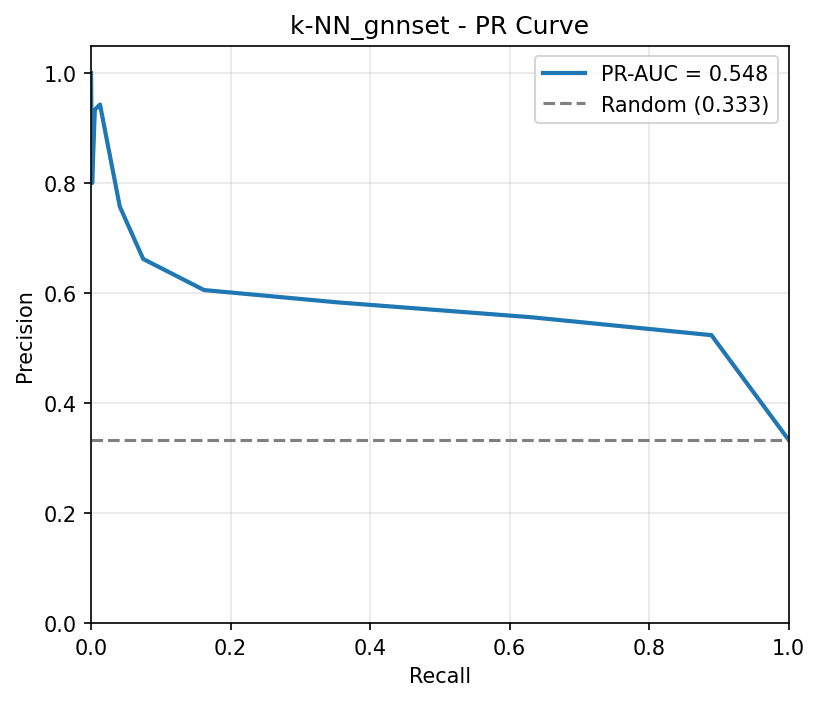
\includegraphics[width=0.48\textwidth]{figures/k-NN_pr.png}\hfill
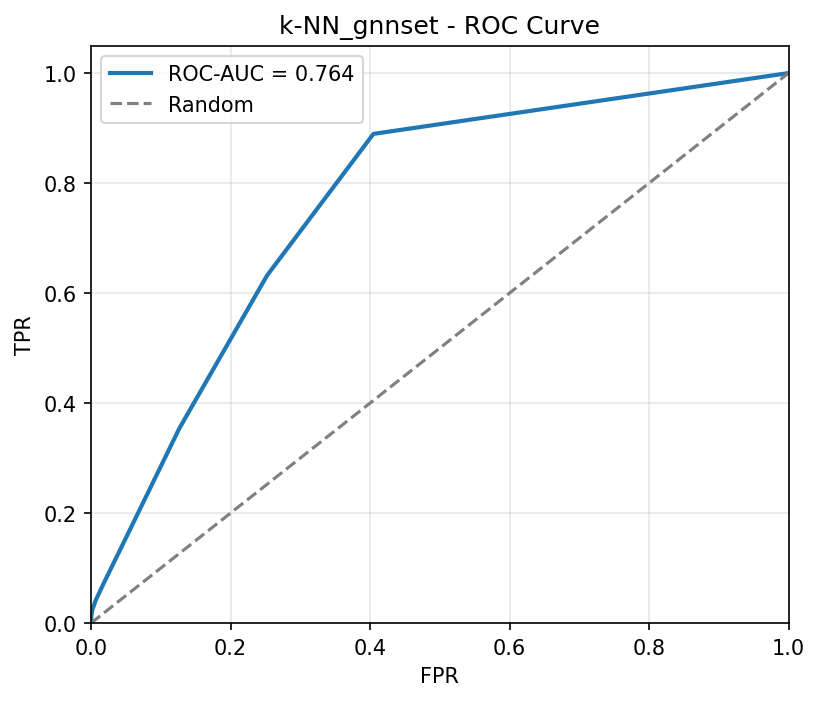
\includegraphics[width=0.48\textwidth]{figures/k-NN_roc.png}
\caption{Krzywa PR i~ROC klasyfikatora k-NN ($k{=}10$) na zbiorze testowym.}
\label{fig:knn_curves}
\end{figure}

\begin{figure}[htbp]
\centering
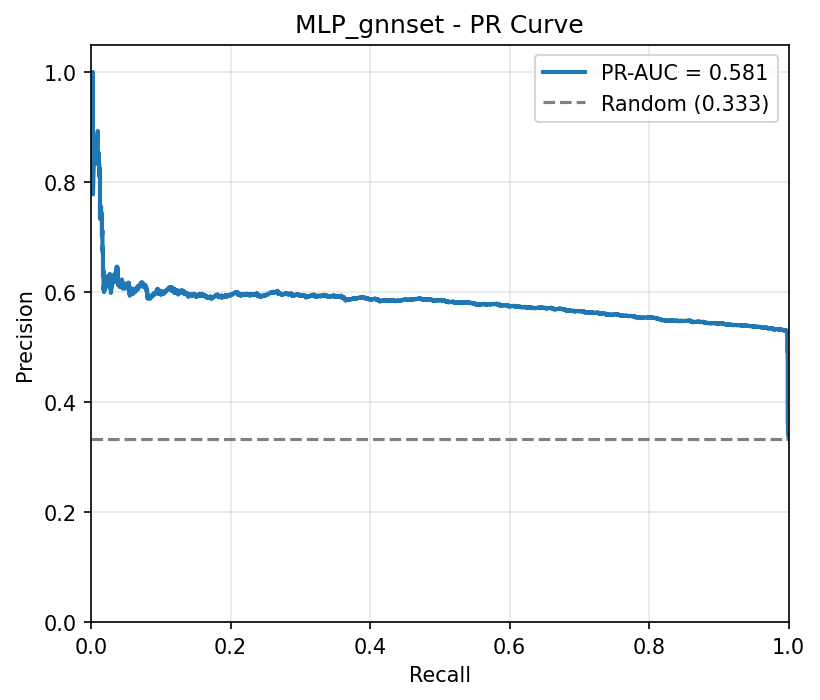
\includegraphics[width=0.48\textwidth]{figures/MLP_pr.png}\hfill
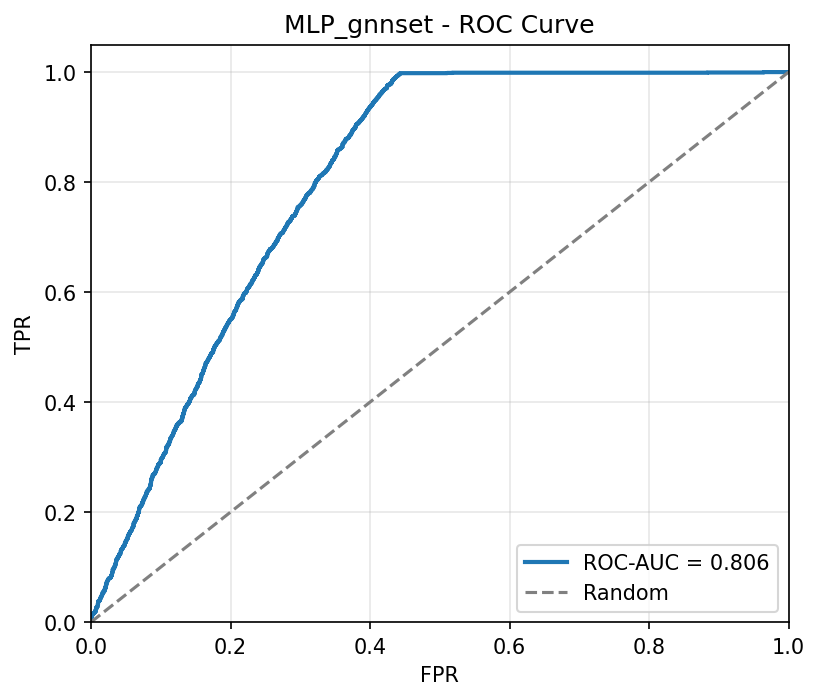
\includegraphics[width=0.48\textwidth]{figures/MLP_roc.png}
\caption{Krzywa PR i~ROC modelu MLP na zbiorze testowym.}
\label{fig:mlp_curves}
\end{figure}

\begin{figure}[htbp]
\centering
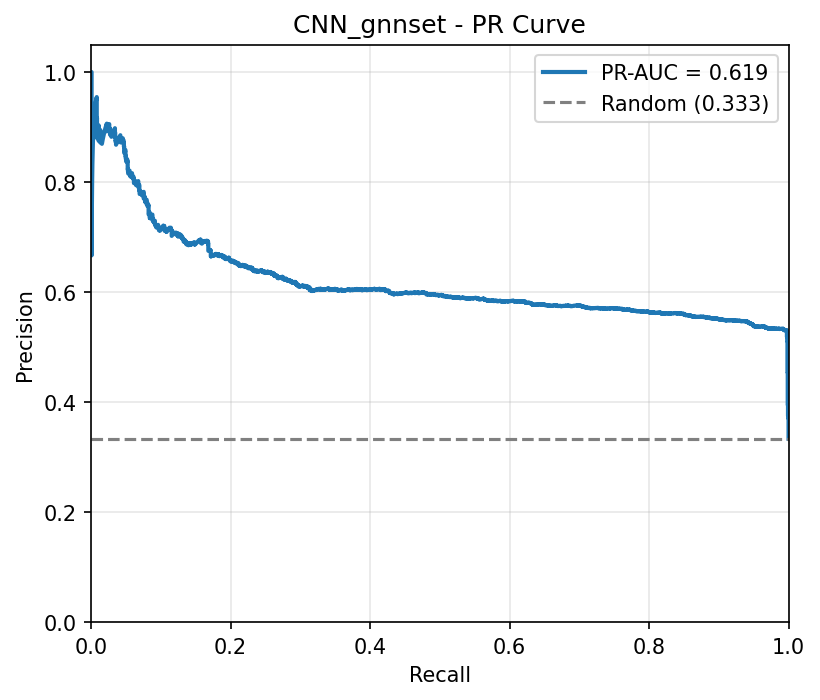
\includegraphics[width=0.48\textwidth]{figures/CNN_pr.png}\hfill
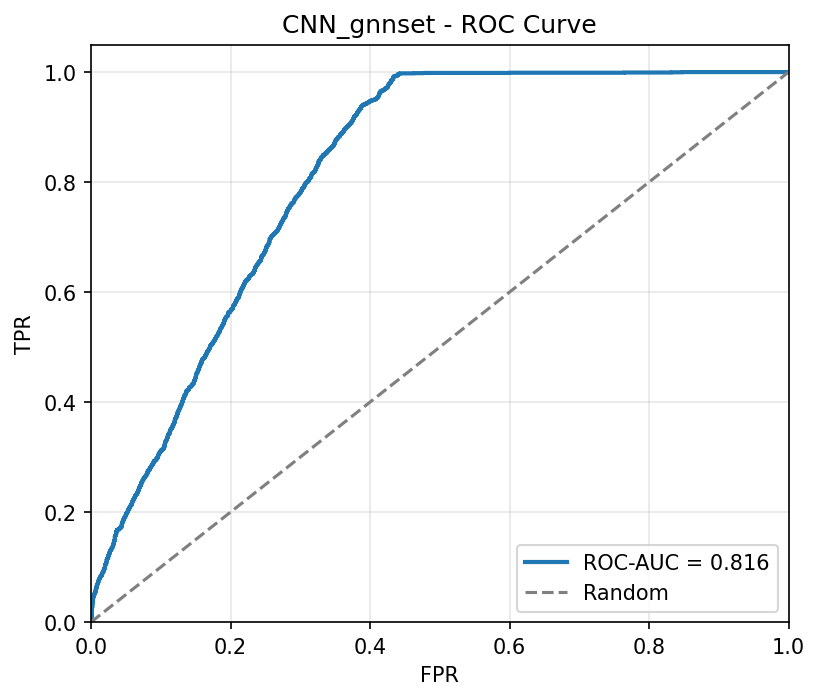
\includegraphics[width=0.48\textwidth]{figures/CNN_roc.png}
\caption{Krzywa PR i~ROC modelu CNN na zbiorze testowym.}
\label{fig:cnn_curves}
\end{figure}

\begin{figure}[htbp]
\centering
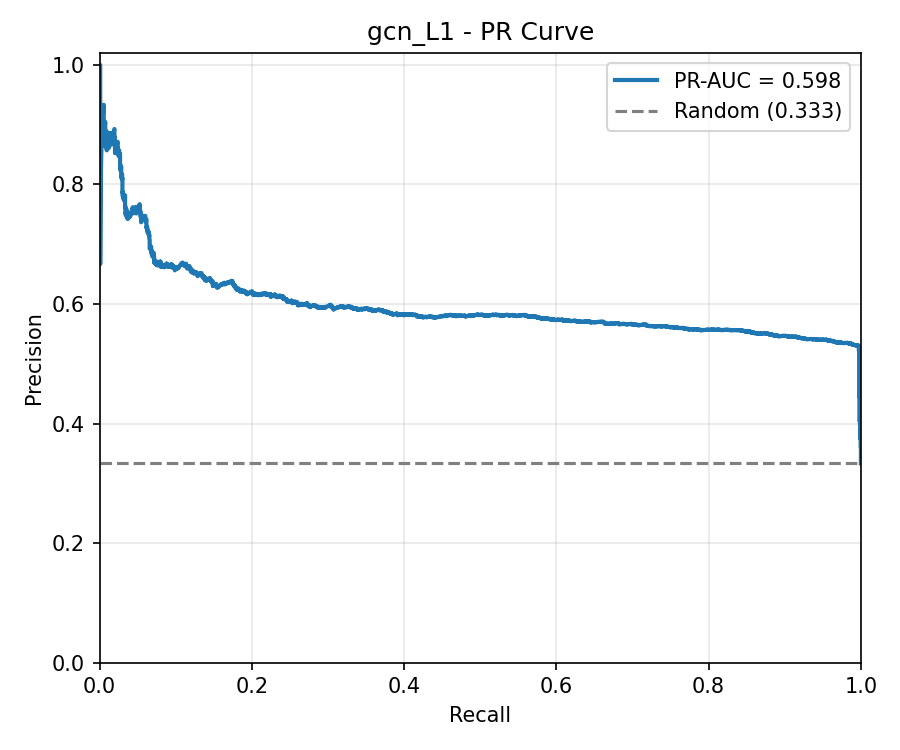
\includegraphics[width=0.48\textwidth]{figures/gcn_L1_pr.png}\hfill
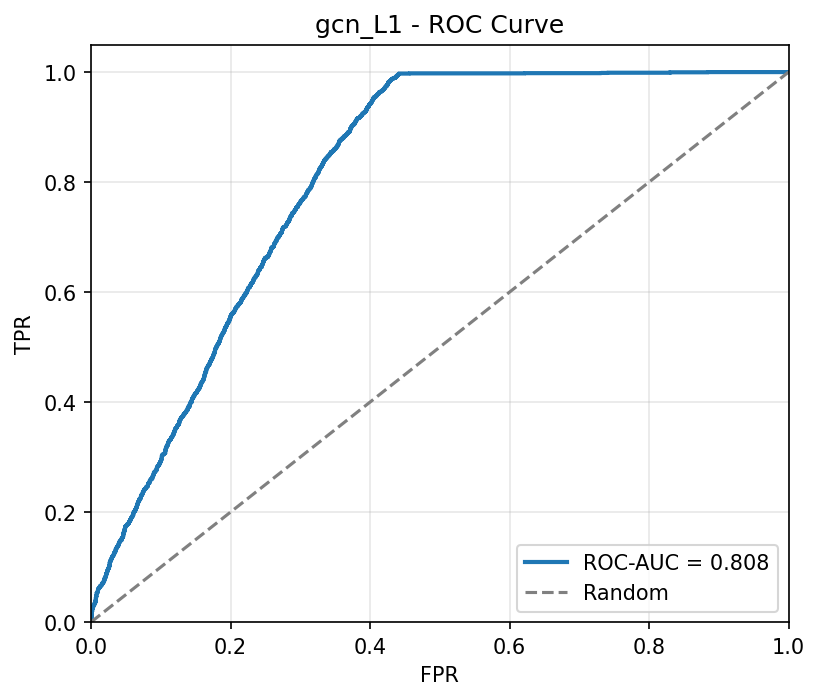
\includegraphics[width=0.48\textwidth]{figures/gcn_L1_roc.png}
\caption{Krzywa PR i~ROC modelu GNN (GCNConv $L{=}1$, najlepszy wariant ablation study)
na zbiorze testowym przy rzeczywistej proporcji pozytywów ${\approx}33\%$.}
\label{fig:gnn_curves}
\end{figure}

\begin{figure}[htbp]
\centering
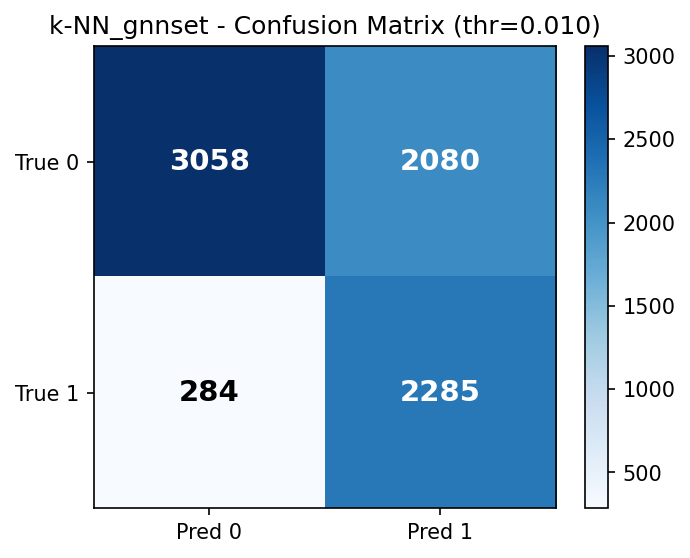
\includegraphics[width=0.48\textwidth]{figures/k-NN_cm.png}\hfill
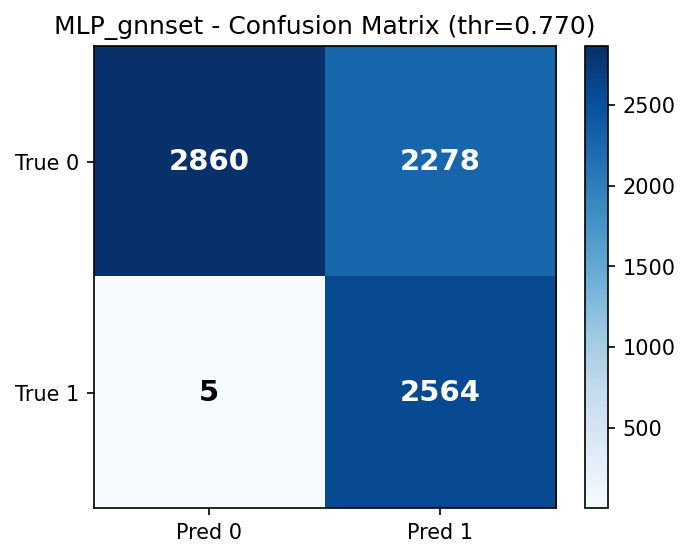
\includegraphics[width=0.48\textwidth]{figures/MLP_cm.png}\\[6pt]
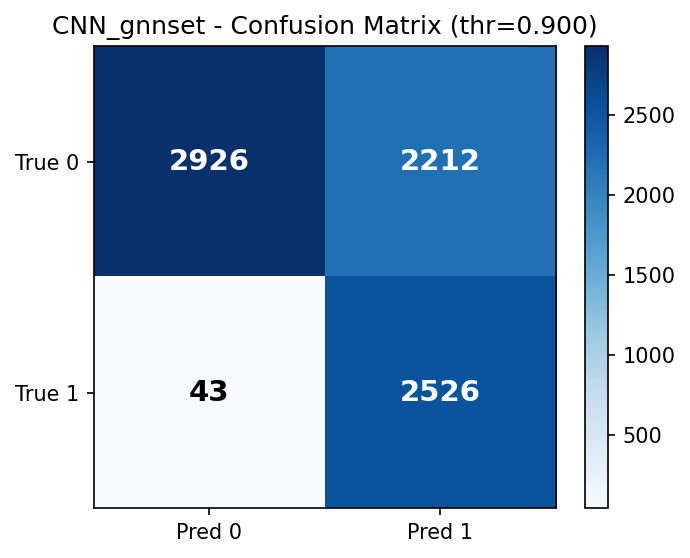
\includegraphics[width=0.48\textwidth]{figures/CNN_cm.png}\hfill
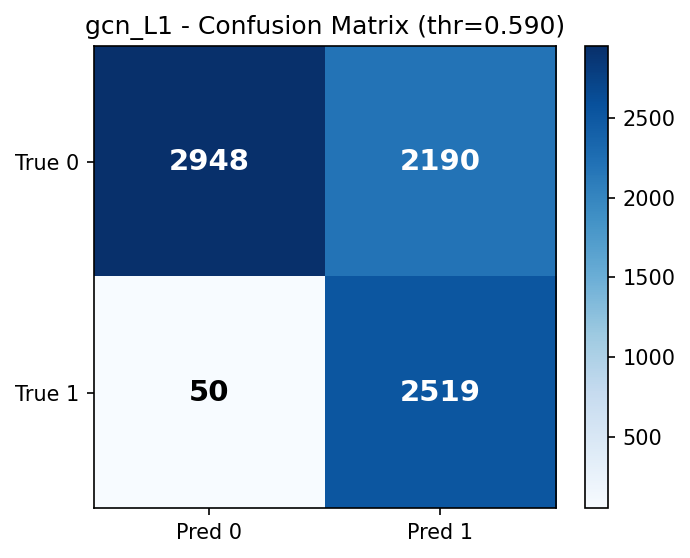
\includegraphics[width=0.48\textwidth]{figures/gcn_L1_cm.png}
\caption{Macierze pomyłek na zbiorze testowym ($n{=}7707$) przy progu F1 dobranym na zbiorze walidacyjnym: k-NN (góra lewo),
MLP (góra prawo), CNN (dół lewo), GNN GCNConv $L{=}1$ (dół prawo).}
\label{fig:confusion_matrices}
\end{figure}

\subsection{Istotność różnic między modelami}
\label{sec:diff_ci}

Porównanie samych wartości punktowych nie wystarcza do oceny, czy obserwowana przewaga jednego
modelu nad drugim jest istotna statystycznie. Często stosowane kryterium nakładania się
\textit{brzegowych} przedziałów ufności obu modeli jest przy tym mylące: dwa estymatory mogą mieć
nakładające się brzegowe CI, a~mimo to różnica między nimi może być istotna~--- decyduje rozkład
\textit{różnicy}, a~nie rozkłady brzegowe~\cite{efron1979}.

Z~tego powodu zastosowano \textbf{sparowany bootstrap różnicy}: w~każdej z~1000~iteracji losuje się
(ze~zwracaniem) jeden wspólny zbiór indeksów próby testowej, a~następnie oblicza różnicę metryki
między dwoma modelami ocenianymi na \textit{tej samej} podpróbie. Wyznaczone w~ten sposób różnice
i~ich 95\%~przedziały ufności zestawia tabela~\ref{tab:diff_ci}.

\begin{table}[htbp]
\centering
\small
\caption{Sparowany bootstrap różnic metryk (1000~iteracji, jednolity zbiór testowy $n{=}7707$).
Dodatnia wartość oznacza przewagę CNN. Przedziały ufności wykluczające zero wskazują na
statystycznie istotną różnicę.}
\label{tab:diff_ci}
\begin{tabular}{lcc}
\toprule
\textbf{Porównanie} & \textbf{$\Delta$PR-AUC [95\% CI]} & \textbf{$\Delta$ROC-AUC [95\% CI]} \\
\midrule
CNN $-$ MLP & $+0{,}038\ [+0{,}021;\ +0{,}054]$ & $+0{,}010\ [+0{,}003;\ +0{,}017]$ \\
CNN $-$ GNN & $+0{,}022\ [+0{,}006;\ +0{,}037]$ & $+0{,}008\ [+0{,}001;\ +0{,}015]$ \\
\bottomrule
\end{tabular}
\end{table}

Wszystkie cztery przedziały ufności różnic wykluczają zero, co oznacza, że przewaga CNN nad
MLP oraz nad GNN jest istotna statystycznie w~obu metrykach. Należy jednak podkreślić, że
\textbf{rozmiar tego efektu jest niewielki} (różnice ROC-AUC rzędu $0{,}008$--$0{,}010$), a~wyniki
pochodzą z~pojedynczego przebiegu treningowego (sekcja~\ref{sec:limitations}). Wniosek o~przewadze
CNN należy zatem traktować z~ostrożnością: jest on statystycznie wykrywalny na tym zbiorze, lecz
jego praktyczne znaczenie pozostaje ograniczone.

\subsection{Analiza progów decyzyjnych}
\label{sec:thresholds}

Wyjściem każdego modelu (poza k-NN) jest logit $s$, przekształcany sigmoidą na prawdopodobieństwo
wiązania $\hat{p} = \sigma(s) \in [0,1]$, które dla uzyskania twardej decyzji binarnej należy poddać progowaniu. Wartości metryk rankingowych
(PR-AUC, ROC-AUC) są niezależne od progu, natomiast $F_1$, MCC i~macierz pomyłek zależą od jego
wyboru. W~niniejszej pracy próg $\theta^*$ dobierano \textbf{wyłącznie na zbiorze walidacyjnym}
przez maksymalizację $F_1$, a~następnie stosowano go bez zmian na zbiorze testowym~--- procedura ta
zapobiega optymistycznemu obciążeniu wynikającemu z~dostrajania progu do danych testowych.

Wyznaczone progi $\theta^*$ różnią się znacząco między modelami (tabela~\ref{tab:thresholds}),
co odzwierciedla odmienną kalibrację ich wyjść. Model CNN wymaga wysokiego progu ($\theta^* = 0{,}90$),
gdyż jego rozkład prawdopodobieństw jest przesunięty ku wysokim wartościom; GNN i~MLP osiągają
optimum przy progach pośrednich ($0{,}59$ i~$0{,}77$). Mimo tych różnic uzyskiwane wartości $F_1$
i~MCC są bardzo zbliżone (tabela~\ref{tab:thresholds}), co wskazuje, że po właściwej kalibracji
progu modele neuronowe oferują porównywalną jakość klasyfikacji binarnej. Niska wartość progu dla
k-NN ($0{,}01$) wynika z~dyskretnego charakteru jego wyjścia (frakcja $k{=}10$ sąsiadów), co czyni
ten model najmniej elastycznym w~kontroli kompromisu precyzja--czułość.

\begin{table}[htbp]
\centering
\small
\caption{Optymalne progi decyzyjne $\theta^*$ (dobrane na zbiorze walidacyjnym przez maksymalizację
$F_1$) oraz odpowiadające im wartości $F_1$ i~MCC na zbiorze testowym.}
\label{tab:thresholds}
\begin{tabular}{lccc}
\toprule
\textbf{Model} & \textbf{$\theta^*$} & \textbf{$F_1$} & \textbf{MCC} \\
\midrule
k-NN ($k{=}10$)      & $0{,}01$ & $0{,}659$ & $0{,}461$ \\
MLP                  & $0{,}77$ & $0{,}692$ & $0{,}541$ \\
CNN (NetTCR-2.0)     & $0{,}90$ & $0{,}691$ & $0{,}535$ \\
GNN (GCNConv $L{=}1$) & $0{,}59$ & $0{,}692$ & $0{,}536$ \\
\bottomrule
\end{tabular}
\end{table}

\subsection{Ewaluacja w obrębie pojedynczego allelu HLA-A*03:01}
\label{sec:within_allele}

Zbiór roboczy obejmuje dwa allele MHC: HLA-A*03:01 (${\approx}20{,}7\%$ pozytywów)
oraz HLA-A*24:02 (${\approx}0{,}04\%$ pozytywów; 30 na 66~957 par). Tak skrajna
asymetria wynika ze~składu danych: w~zbiorze IE-1\_CMV kompleks \texttt{AYAQKIFKI}/HLA-A*24:02
jest reprezentowany niemal wyłącznie przez obserwacje negatywne (30~pozytywów na ${\approx}67\,000$~par),
wskutek czego pary $(\text{TCR},\ \text{A*24:02})$ są w~praktyce niemal zawsze negatywne,
niezależnie od sekwencji TCR. Oznacza to, że
metryki agregatowe z~tabeli~\ref{tab:results} łączą \textit{dwa} zadania o~różnej
trudności: trywialne rozróżnienie allelu prezentującego oraz właściwą predykcję
specyficzności TCR \textit{w~obrębie} allelu prezentującego.

Skalę tego zjawiska ilustruje prosty test: predyktor korzystający \textbf{wyłącznie}
z~tożsamości allelu (przypisujący każdej parze treningowy odsetek pozytywów dla danego
allelu, ignorujący całkowicie TCR) osiąga na zbiorze agregatowym ROC-AUC ${=}0{,}777$
oraz PR-AUC ${=}0{,}529$~--- a~zatem dorównuje pełnemu klasyfikatorowi k-NN, a~w~ROC-AUC
nawet go przewyższa. Znaczna część pozornej jakości modeli odzwierciedla więc
rozróżnienie allelu, a~nie rozpoznawanie wzorców wiązania TCR.

Aby wyodrębnić sygnał zależny wyłącznie od TCR, ograniczono ewaluację do par
z~allelem HLA-A*03:01 ($n{=}4841$, ${\approx}53\%$ pozytywów). W~tym podzbiorze cecha MHC
jest stała, więc~--- jako że ROC-AUC i~PR-AUC są metrykami rankingowymi~--- wkład allelu
sprowadza się do stałego przesunięcia identycznego dla wszystkich próbek i~nie wpływa na
ich wartości. Otrzymane liczby (tabela~\ref{tab:within_allele}) mierzą zatem czystą
zdolność tych samych, wytrenowanych modeli do rozróżniania wiążących i~niewiążących TCR.

\begin{table}[htbp]
\centering
\small
\caption{Porównanie metryk na zbiorze agregatowym (oba allele, tabela~\ref{tab:results})
oraz w~obrębie samego allelu prezentującego HLA-A*03:01 ($n{=}4841$, ${\approx}53\%$
pozytywów). Po odizolowaniu trywialnego rozróżnienia allelu ROC-AUC zapada się z~0{,}76--0{,}82
do 0{,}55--0{,}59. Różne wartości bazowe PR-AUC (0{,}333 vs.\ 0{,}530) wynikają z~odmiennego
odsetka pozytywów, dlatego porównania między zbiorami należy opierać na ROC-AUC.}
\label{tab:within_allele}
\begin{tabular}{lcccc}
\toprule
\textbf{Model} & \multicolumn{2}{c}{\textbf{ROC-AUC}} & \multicolumn{2}{c}{\textbf{PR-AUC}} \\
\cmidrule(lr){2-3}\cmidrule(lr){4-5}
                      & agreg. & A*03:01 & agreg. & A*03:01 \\
\midrule
Klas.\ losowy         & $0{,}500$ & $0{,}500$ & $0{,}333$ & $0{,}530$ \\
k-NN ($k{=}10$)       & $0{,}764$ & $0{,}550$ & $0{,}548$ & $0{,}574$ \\
MLP                   & $0{,}806$ & $0{,}565$ & $0{,}581$ & $0{,}581$ \\
CNN (NetTCR-2.0)      & $0{,}816$ & $0{,}588$ & $0{,}619$ & $0{,}620$ \\
GNN (GCNConv $L{=}1$) & $0{,}808$ & $0{,}571$ & $0{,}598$ & $0{,}598$ \\
\bottomrule
\end{tabular}
\end{table}

Wyniki prowadzą do trzech wniosków. Po pierwsze, sygnał zależny od TCR jest
\textbf{realny, lecz skromny}: wszystkie modele pozostają istotnie powyżej poziomu
losowego (95\%~CI dla ROC-AUC w~obrębie A*03:01 wykluczają 0{,}5: k-NN $[0{,}534;\ 0{,}566]$,
MLP $[0{,}548;\ 0{,}582]$, CNN $[0{,}571;\ 0{,}604]$, GNN $[0{,}555;\ 0{,}586]$). Po drugie,
\textbf{hierarchia modeli zostaje zachowana} (CNN $>$ GNN $>$ MLP $>$ k-NN); mierzona
przyrostem PR-AUC ponad poziom losowy wynosi ona odpowiednio $+0{,}090$, $+0{,}068$,
$+0{,}052$ i~$+0{,}045$, a~modele neuronowe wyciągają z~sekwencji TCR około dwukrotnie
więcej sygnału niż baseline k-NN. Po trzecie, dystans między najlepszym modelem a~k-NN
jest na właściwym zadaniu \textit{większy} niż sugerują metryki agregatowe, co dodatkowo
wspiera wniosek z~sekcji~\ref{sec:diff_ci}.

Ponieważ wszystkie modele trenowano na obu allelach, ograniczenie ewaluacji do
HLA-A*03:01 izoluje sygnał TCR \textit{bez} ponownego treningu. Kierunek ewentualnego
obciążenia jest przy tym korzystny dla powyższej interpretacji: trywialne negatywy
z~allelu A*24:02 mogą jedynie \textit{rozcieńczać}, a~nie zawyżać sygnał wewnątrz allelu,
zatem podane wartości są konserwatywne. Potwierdza to kontrola, w~której klasyfikator k-NN
trenowano \textit{wyłącznie} na parach z~HLA-A*03:01: uzyskuje on ROC-AUC ${=}0{,}550$~---
identyczne jak przy treningu na obu allelach~--- co dowodzi, że skład zbioru treningowego
nie wpływa istotnie na ocenę w~obrębie allelu.

\subsection{Wpływ schematu ważenia klas (ablacja)}
\label{sec:weighting_ablation}

W~odpowiedzi na pytanie o~możliwe podwójne ważenie klasy pozytywnej przeprowadzono ablację
dla modelu MLP w~trzech reżimach: wyłącznie zbalansowane próbkowanie, wyłącznie waga $w_+$
oraz oba mechanizmy łącznie (konfiguracja użyta w~pracy). Ewaluację wykonano na zbiorze
testowym o~rozkładzie naturalnym, przy progu dobranym na walidacji.

\begin{table}[htbp]
\centering
\small
\caption{Wpływ schematu ważenia klas na MLP (zbiór testowy, rozkład naturalny). Metryki
rankingowe (PR-AUC, ROC-AUC) są praktycznie identyczne między reżimami (różnice w~granicach
przedziałów ufności). Punkt pracy (czułość, liczba fałszywie pozytywnych FP, $F_1$) jest również
zbliżony we~wszystkich trzech reżimach, co pokazuje, że wysoka czułość nie jest skutkiem łącznego
ważenia, lecz progu $F_1$ na niezrównoważonym zbiorze.}
\label{tab:weighting}
\begin{tabular}{lcccccc}
\toprule
\textbf{Reżim} & \textbf{PR-AUC} & \textbf{ROC-AUC} & \textbf{Czułość} & \textbf{FP} & \textbf{F1} & \textbf{Próg $\theta^*$} \\
\midrule
Sampler only      & $0{,}250$ & $0{,}804$ & $0{,}998$ & $9617$ & $0{,}348$ & $0{,}40$ \\
$w_+$ only         & $0{,}239$ & $0{,}796$ & $0{,}998$ & $9615$ & $0{,}348$ & $0{,}46$ \\
Sampler $+\ w_+$ (użyty) & $0{,}248$ & $0{,}801$ & $0{,}998$ & $9616$ & $0{,}348$ & $0{,}69$ \\
\bottomrule
\end{tabular}
\end{table}

Wyniki prowadzą do dwóch wniosków. Po pierwsze, schemat ważenia nie zniekształca metryk
rankingowych, na których opierają się wnioski pracy~--- PR-AUC i~ROC-AUC pozostają w~granicach
przedziałów ufności niezależnie od konfiguracji. Po drugie, wysoka czułość i~liczba fałszywie
pozytywnych nie są artefaktem \emph{łącznego} ważenia: występują w~podobnej skali także przy
pojedynczym mechanizmie i~wynikają z~doboru progu maksymalizującego $F_1$ przy silnym
niezrównoważeniu klas. Ważenie zmienia natomiast \emph{kalibrację} modelu: optymalny próg
$\theta^*$ rośnie z~$0{,}40$ (sam sampler) do~$0{,}69$ (oba mechanizmy), a~ponieważ próg dobierany
jest na zbiorze walidacyjnym, ta różnica zostaje pochłonięta~--- stąd niemal identyczny punkt
pracy mimo odmiennego schematu ważenia. Punkt pracy można w~razie potrzeby przesunąć ku wyższej
precyzji, dobierając próg pod kątem innej miary (np.\ MCC) lub konkretnego zastosowania.

% ============================================================
\chapter{Zakończenie}
\label{chap:zakonczenie}
% ============================================================

\section{Podsumowanie wyników}

Niniejsza praca postawiła sobie za cel systematyczne porównanie czterech klas metod uczenia
maszynowego w~zadaniu binarnej predykcji wiązania TCR-pMHC na przykładzie immunodominującego
epitopu IE-1 wirusa CMV. Wszystkie modele ewaluowano przy użyciu PR-AUC jako głównej metryki~---
adekwatnej dla silnie niezrównoważonych danych biologicznych~\cite{davis2006}~---
oraz ROC-AUC uzupełniająco, w~celu porównywalności z~literaturą.

Wyniki (tabela~\ref{tab:results}) ujawniają spójną hierarchię w~obu metrykach. W~ROC-AUC
wszystkie trzy modele neuronowe (MLP, CNN, GNN) przewyższają k-NN (0,806--0,816 vs.\ 0,764),
natomiast różnice między modelami neuronowymi są małe: CNN = 0,816, GNN = 0,808, MLP = 0,806.
W~PR-AUC kolejność jest zbliżona: CNN = 0,619, GNN = 0,598, MLP = 0,581, k-NN = 0,548
(przy bazowej wartości losowej 0,333). Brzegowe przedziały ufności CNN i~GNN częściowo się
nakładają (w~PR-AUC $[0{,}599;\ 0{,}641]$ vs.\ $[0{,}578;\ 0{,}619]$), nakładanie brzegowych CI
nie jest jednak właściwym kryterium istotności różnicy między modelami. Sparowany bootstrap
\textit{różnicy} (sekcja~\ref{sec:diff_ci}), w~którym w~każdej iteracji ta sama wylosowana próba
ocenia oba modele, wskazuje, że przewaga CNN nad GNN jest statystycznie istotna (CI różnicy
wyklucza zero), choć o~niewielkim rozmiarze efektu. Wobec pojedynczego ziarna losowości
(sekcja~\ref{sec:limitations}) wynik ten wymaga ostrożnej interpretacji.

Aby zapewnić porównywalność wyników, wszystkie modele ewaluowano na tym samym zbiorze testowym
($n{=}7707$) odpowiadającym podgrafom GNN. Zbiór ten zawiera wszystkie pozytywy oraz
dwukrotną losową próbkę negatywów (${\approx}33\%$ pozytywów). Wcześniejsza wersja pracy
raportowała zawyżone wartości PR-AUC modeli sekwencyjnych wskutek błędnego użycia
WeightedRandomSampler na loaderze testowym; obecne wyniki zostały poprawione i~ujednolicone.

Należy jednak podkreślić, że metryki agregatowe (tabela~\ref{tab:results}) łączą dwa
zadania o~różnej trudności. Ponieważ allel HLA-A*24:02 jest w~zbiorze reprezentowany niemal wyłącznie przez negatywy,
znaczna część wysokich wartości ROC-AUC (0{,}76--0{,}82) odzwierciedla trywialne
rozróżnienie allelu, a~nie specyficzność TCR. Po ograniczeniu ewaluacji do samego allelu
prezentującego (sekcja~\ref{sec:within_allele}) ROC-AUC zapada się do 0{,}55--0{,}59,
ujawniając rzeczywisty, lecz skromny sygnał TCR. Hierarchia modeli i~przewaga CNN
pozostają przy tym w~mocy, co czyni główny wniosek porównawczy pracy odpornym na ten
artefakt doboru danych. Dla pełnego obrazu w~tabeli~\ref{tab:natural} podano wyniki na
naturalnym rozkładzie klas (${\approx}10{,}6\%$ pozytywów): bezwzględne PR-AUC spada wówczas do
${\approx}0{,}24$--$0{,}30$ (poziom losowy $0{,}106$), co potwierdza, że praktyczna jakość modeli
jest skromna, choć ranking CNN $>$ MLP $>$ k-NN pozostaje zachowany. Za właściwą miarę zdolności
rozpoznawania TCR należy zatem przyjąć ewaluację w~obrębie allelu prezentującego
(sekcja~\ref{sec:within_allele}), a~nie metryki agregatowe.

Przebiegi ablacyjne GNN z~głębokościami $L \in \{1, 2, 3, 4\}$ (tabela~\ref{tab:ablation_gnn})
wskazują na stabilność procedury optymalizacji~--- różnice PR-AUC i~ROC-AUC między konfiguracjami
są nieduże, a~wariant $L{=}1$ osiąga najwyższą wartość PR-AUC (0,598).
Na jednolitym zbiorze testowym GNN (PR-AUC = 0,598) nie przewyższa najlepszego modelu
sekwencyjnego~--- CNN (0,619); sparowany bootstrap potwierdza istotną, choć niewielką,
przewagę CNN. Hipoteza zerowa H$_0$~--- że architektura grafowa z~grafem k-NN sąsiedztwa
nie wnosi istotnej przewagi predykcyjnej nad prostszymi modelami sekwencyjnymi~--- pozostaje
zatem w~mocy. Brak przewagi GNN nad modelami
sekwencyjnymi można wyjaśnić kilkoma mechanizmami. Po pierwsze, embeddingi ESM2 mogą już
enkodować biologiczne sąsiedztwo w~przestrzeni sekwencji, co czyni agregację grafową
w~znacznym stopniu redundantną. Po drugie, graf k-NN konstruowany w~przestrzeni tych samych
embeddingów nie wnosi informacji ortogonalnej wobec samych reprezentacji. Po trzecie, przy
ograniczonej liczbie pozytywnych obserwacji (${\approx}8800$ w~zbiorze treningowym) model
może nie mieć wystarczającej ilości danych, by nauczyć się nietrywialnej propagacji przez
graf.

\section{Dyskusja}

\subsection{Odniesienie do literatury}

Opublikowane wyniki dla porównywalnych zadań predykcji TCR-pMHC wskazują na wartości
ROC-AUC rzędu 0{,}85--0{,}92 i~PR-AUC rzędu 0{,}55--0{,}75 dla modeli wykorzystujących sparowane
łańcuchy $\alpha$/$\beta$~\cite{montemurro2022,springer2020,weber2021}. NetTCR-2.0~\cite{montemurro2022}
osiąga ROC-AUC $\approx 0{,}85$ na danych CMV dla modelu splotowego z~oboma łańcuchami. Praca TITAN~\cite{weber2021}
stosuje dwumodalne sieci uwagi, osiągając porównywalną jakość na zbiorach IEDB i~VDJdb.

Bezpośrednie porównania wartości bezwzględnych są jednak utrudnione przez różnice
w~doborze negatywów między zbiorami. Raportowane w~niniejszej pracy metryki agregatowe
(ROC-AUC ${\approx}0{,}82$) zawyża obecność niemal wyłącznie negatywnego allelu HLA-A*24:02; po
ograniczeniu do allelu prezentującego (sekcja~\ref{sec:within_allele}) ROC-AUC spada do
0{,}55--0{,}59, co sugeruje, że również zewnętrzne wyniki literaturowe mogą być wrażliwe
na analogiczne decyzje konstrukcyjne dotyczące zbioru negatywów.

Kluczową różnicą niniejszej pracy w~stosunku do wymienionych publikacji jest zastosowanie \textit{sparowanych}
sekwencji $\alpha$ i~$\beta$ z~bazy TRAIT, co jest rzadkością w~literaturze. Wiele opublikowanych
modeli, w~tym wczesne wersje NetTCR, opierało się wyłącznie na łańcuchu $\beta$. Dostępność par
$(\alpha, \beta)$ powinna sprzyjać wyższej precyzji predykcji~\cite{montemurro2022}.

\subsection{Ograniczenia badania}
\label{sec:limitations}

Niniejsza praca ma kilka istotnych ograniczeń:

\begin{enumerate}
  \item \textbf{Jeden epitop.} Wyniki dotyczą wyłącznie epitopu IE-1 w~kontekście dwóch alleli
        HLA. Zdolność modeli do generalizacji na inne epitopy i~allele MHC nie była testowana,
        a~predykcja TCR-pMHC jest silnie specyficzna dla konkretnych par peptyd-MHC~\cite{moris2021}.

  \item \textbf{Heurystyka oparta na allelu i~dobór negatywów.} Allel HLA-A*03:01
        dostarcza ${\approx}99{,}8\%$ sygnału pozytywnego, podczas gdy retencjonowany
        w~zbiorze allel HLA-A*24:02 jest reprezentowany niemal wyłącznie przez obserwacje
        negatywne i~stanowi zbiór negatywów trywialnie odróżnialnych po samej tożsamości allelu. Wskutek tego metryki
        agregatowe są zawyżone: predyktor ignorujący TCR i~korzystający wyłącznie
        z~allelu osiąga ROC-AUC 0{,}777. Po odizolowaniu tego artefaktu (ewaluacja
        w~obrębie HLA-A*03:01, sekcja~\ref{sec:within_allele}) rzeczywista zdolność
        rozróżniania TCR okazuje się skromna (ROC-AUC 0{,}55--0{,}59), choć istotnie
        powyżej poziomu losowego, a~hierarchia modeli pozostaje zachowana. Bardziej
        rygorystyczny protokół wykluczałby allel pozbawiony sygnału pozytywnego lub
        stosował trudniejsze negatywy (np.\ wymianę TCR w~obrębie allelu prezentującego).

  \item \textbf{Brak zewnętrznych baz danych.} Dane z~VDJdb, IEDB i~McPAS-TCR nie zostały
        włączone, co ogranicza zewnętrzną trafność wyników i~uniemożliwia ocenę zdolności
        transferu wiedzy między bazami.

  \item \textbf{Prymitywna topologia grafu.} Graf k-NN oparty na podobieństwie embeddingów
        ESM2 jest prostym przybliżeniem biologicznego sąsiedztwa. Bardziej informacyjne mogłyby
        być grafy oparte na podobieństwie strukturalnym CDR3 w~3D, oddziaływaniach
        TCR-pMHC ze~struktur krystalograficznych lub epitopowej specyficzności z~dedykowanych
        baz danych.

  \item \textbf{\textit{Cross}-reaktywność.} Model nie uwzględnia wprost zdolności jednego TCR do
        rozpoznawania wielu epitopów (\textit{cross-reactivity}), co jest biologicznie istotnym
        aspektem specyficzności TCR.

  \item \textbf{Pojedyncze ziarno losowości.} Każdy model trenowano w~jednym przebiegu z~ustalonym
        ziarnem (\texttt{seed = 42}). Przy różnicach ROC-AUC rzędu $0{,}008$--$0{,}010$ między
        modelami neuronowymi wariancja wynikająca z~inicjalizacji wag i~kolejności próbkowania
        może być porównywalna z~obserwowanymi różnicami. Choć sparowany bootstrap różnic
        (sekcja~\ref{sec:diff_ci}) kontroluje niepewność wynikającą z~\textit{doboru próby
        testowej}, nie obejmuje on wariancji \textit{procedury treningowej}. Pełne potwierdzenie
        rankingu modeli wymagałoby kilku niezależnych przebiegów (np.\ 3--5~ziaren) i~raportowania
        średniej wraz z~odchyleniem standardowym~--- co pozostawiono jako kierunek dalszych prac.

  \item \textbf{Łączne ważenie klas.} Zastosowano jednocześnie zbalansowane próbkowanie
        i~wagę $w_+$ w~stracie. Ablacja (sekcja~\ref{sec:weighting_ablation},
        tabela~\ref{tab:weighting}) potwierdza, że schemat ważenia nie wpływa istotnie na
        PR-AUC/ROC-AUC ani na punkt pracy; wysoka czułość wynika z~progu $F_1$ na niezrównoważonym
        zbiorze, a~nie z~podwójnego ważenia.

  \item \textbf{Bootstrap na poziomie obserwacji.} Przedziały ufności wyznaczono, próbkując
        pojedyncze obserwacje. Ponieważ ten sam TCR może pojawiać się w~wielu parach, bardziej
        konserwatywny byłby \emph{cluster bootstrap} po unikatowych TCR; obecne CI mogą
        nieznacznie niedoszacowywać niepewności.
\end{enumerate}

\section{Kierunki przyszłych badań}

Na podstawie doświadczeń zebranych w~niniejszej pracy proponuje się następujące kierunki dalszych
prac:

\begin{enumerate}
  \item \textbf{Rozszerzenie na wiele epitopów chorobowych.} Niniejsza praca skupia się
        wyłącznie na epitopie IE-1 wirusa CMV. Naturalnym rozszerzeniem jest włączenie
        epitopów innych patogenów (np.\ EBV (\textit{Epstein-Barr virus}), HIV, SARS-CoV-2
        czy \textit{Plasmodium falciparum}), które są dobrze scharakteryzowane
        w~bazach VDJdb~\cite{bagaev2020} i~McPAS-TCR~\cite{tickotsky2017}. Trenowanie na
        wielu epitopach jednocześnie umożliwiłoby ocenę zdolności generalizacji \textit{zero-shot} --
        kluczowego wymogu dla zastosowań klinicznych~\cite{moris2021}.

  \item \textbf{Bardziej zaawansowana topologia grafu.} Obecny graf k-NN oparty wyłącznie
        na podobieństwie kosinusowym embeddingów ESM2 stanowi proste przybliżenie biologicznego
        sąsiedztwa. Bardziej informatywne mogłyby być grafy heterogeniczne łączące węzły TCR
        i~pMHC bezpośrednio, grafy oparte na strukturach 3D kompleksów TCR-pMHC przewidywanych
        przez ESMFold~\cite{lin2023} lub AlphaFold2~\cite{jumper2021}, albo grafy konstruowane
        na podstawie grupowania motywów CDR3 metodami klonotypowania~\cite{glanville2017}.

  \item \textbf{Podejścia hipergrafowe.} Graf k-NN modeluje relacje parami: węzeł TCR łączy
        się z~węzłem TCR. Tymczasem wiązanie TCR-pMHC jest z~natury relacją trójstronną --
        angażuje jednocześnie trzy obiekty: TCR, epitop i~allel MHC. Hipergrafy~\cite{feng2019}
        pozwalają modelować takie relacje wprost: pojedyncza hiperkrawędź 3.~rzędu łączy węzły
        TCR, Epitop i~MHC jako jeden obiekt relacyjny. Hipergrafowa sieć neuronowa (HGNN)
        propagowałaby informację wzdłuż tych trójstronnych hiperkrawędzi, umożliwiając globalną
        agregację wiedzy o~tym, które pary TCR-MHC są zdolne do wiązania danego epitopu, bez
        konieczności sprowadzania problemu do relacji binarnych.

  \item \textbf{Lepsze reprezentacje MHC.} Zastosowanie embeddingów pełnej pseudosekwencji MHC
        lub dedykowanego kodera allelu opartego na ESM2, który może lepiej uchwytywać
        ograniczenia allelu przy predykcji na nowych allelach~\cite{montemurro2022}.

  \item \textbf{Uczenie kontrastywne.} Pretrenowanie modeli na zadaniu rozróżniania par TCR
        o~podobnym vs.\ odmiennym profilu wiązania jako forma regularyzacji przestrzeni
        embeddingów, potencjalnie poprawiająca jakość reprezentacji przy ograniczonych
        danych pozytywnych~\cite{glanville2017}.
\end{enumerate}

\section{Wnioski}

Niniejsza praca dokumentuje kompleksowe porównanie metodologiczne czterech klas modeli predykcji
TCR-pMHC na jednym z~największych dostępnych zbiorów sparowanych sekwencji TCR dla konkretnego
epitopu wirusowego. Uzyskane wyniki (tabela~\ref{tab:results}) prowadzą do następujących wniosków:
(1)~wszystkie trzy modele neuronowe (MLP, CNN, GNN) przewyższają klasyfikator k-NN
w~obu metrykach (ROC-AUC: 0,806--0,816 vs.\ 0,764; PR-AUC: 0,581--0,619 vs.\ 0,548),
co potwierdza wartość treningu z~nadzorem nad podejściem opartym wyłącznie na podobieństwie;
(2)~GNN (PR-AUC = 0,598, ROC-AUC = 0,808) nie przewyższa modelu splotowego CNN
(PR-AUC = 0,619, ROC-AUC = 0,816), co nie pozwala odrzucić hipotezy zerowej H$_0$ i~wskazuje,
że architektura grafowa z~grafem k-NN sąsiedztwa nie wnosi przewagi nad prostszym modelem
sekwencyjnym na tym zbiorze danych; (3)~CNN uzyskał najwyższą wartość PR-AUC i~ROC-AUC, a~sparowany
bootstrap różnic (tabela~\ref{tab:diff_ci}) potwierdza, że jego przewaga nad MLP i~GNN jest
statystycznie istotna, choć o~niewielkim rozmiarze efektu i~wymagająca ostrożnej interpretacji
wobec pojedynczego ziarna losowości; jest to zgodne z~wynikami literatury dla podobnych
zadań~\cite{montemurro2022}.

Należy jednak zaznaczyć, że powyższe wartości agregatowe są zawyżone przez obecność
niemal wyłącznie negatywnego allelu HLA-A*24:02; po odizolowaniu tego artefaktu (ewaluacja
w~obrębie HLA-A*03:01, sekcja~\ref{sec:within_allele}) rzeczywista zdolność rozróżniania
TCR jest skromna (ROC-AUC 0{,}55--0{,}59), choć istotna statystycznie, a~ustalona
hierarchia modeli pozostaje zachowana. Wniosek porównawczy pracy~--- przewaga modeli
neuronowych nad k-NN oraz brak przewagi GNN nad CNN~--- jest zatem odporny na ten
artefakt doboru danych. Co więcej, na naturalnym rozkładzie klas (tabela~\ref{tab:natural})
bezwzględne PR-AUC modeli jest niskie (${\approx}0{,}24$--$0{,}30$ przy poziomie losowym $0{,}106$),
dlatego praktyczną wartość modeli należy oceniać ostrożnie, opierając wnioski przede wszystkim
na ewaluacji w~obrębie allelu HLA-A*03:01.

Praca stanowi wkład w~dziedzinę obliczeniowej immunoinformatyki poprzez:

\begin{itemize}
  \item dostarczenie systematycznego porównania metod sekwencyjnych i~grafowych w~identycznym
        protokole ewaluacji, z~uwzględnieniem metryki PR-AUC adekwatnej do silnie niezrównoważonych
        danych biologicznych,

  \item szczegółowy opis matematyczny wszystkich zastosowanych architektur (od klasycznej
        k-NN przez konwolucyjną NetTCR-2.0 do grafowej GNN z~mechanizmem podgrafów,
        flagi pozycyjnej (\textit{labeling trick}) i~agregacji JK),

  \item opis kompletnego \textit{pipeline'u} danych: od surowych obserwacji TRAIT przez generowanie
        embeddingów ESM2 i~podział per-TCR do prekomputowanych podgrafów dla GNN,

\end{itemize}


% ============================================================
\begin{thebibliography}{99}

\bibitem{janeway2017}
K.~Murphy, C.~Weaver,
\textit{Janeway's Immunobiology},
wyd.~9, Garland Science, Nowy Jork, 2017. ISBN 978-0-8153-4505-3.

\bibitem{wills1996}
M.~R. Wills, A.~J. Carmichael, K.~Mynard, X.~Jin, M.~P. Weekes, B.~Plachter, J.~G. Sissons,
\textit{The human cytotoxic T-lymphocyte (CTL) response to cytomegalovirus is dominated by structural
protein pp65: frequency, specificity, and T-cell receptor usage of pp65-specific CTL},
Journal of Virology, 70(11):7569--7579, 1996.

\bibitem{sylwester2005}
A.~W. Sylwester, B.~L. Mitchell, J.~B. Edgar, C.~Taormina, C.~Pelte, F.~Ruchti, P.~R. Sleath,
K.~H. Grabstein, N.~A. Hosken, F.~Kern, J.~A. Nelson, L.~J. Picker,
\textit{Broadly targeted human cytomegalovirus-specific CD4$^+$ and CD8$^+$ T~cells dominate the
memory compartments of exposed subjects},
Journal of Experimental Medicine, 202(5):673--685, 2005.

\bibitem{lin2023}
Z.~Lin, H.~Akin, R.~Rao, B.~Hie, Z.~Zhu, W.~Lu, N.~Smetanin, R.~Verkuil, O.~Kabeli, Y.~Shmueli,
A.~Dos Santos Costa, M.~Fazel-Zarandi, T.~Sercu, S.~Candido, A.~Rives,
\textit{Evolutionary-scale prediction of atomic-level protein structure with a~language model},
Science, 379(6637):1123--1130, 2023.

\bibitem{rives2021}
A.~Rives, J.~Meier, T.~Sercu, S.~Goyal, Z.~Lin, J.~Liu, D.~Guo, M.~Ott, C.~L. Zitnick, J.~Ma,
R.~Fergus,
\textit{Biological structure and function emerge from scaling unsupervised learning to 250 million
protein sequences},
Proceedings of the National Academy of Sciences, 118(15):e2016239118, 2021.

\bibitem{montemurro2022}
A.~Montemurro, V.~Schuster, H.~R. Povlsen, A.~K. Bentzen, V.~Jurtz, W.~J. Chronister,
A.~Crinklaw, S.~R. Hadrup, K.~Winther, B.~Peters, N.~Jespersen, M.~Nielsen,
\textit{NetTCR-2.0 enables accurate prediction of TCR-peptide binding by using paired TCR$\alpha$
and $\beta$ sequence data},
Communications Biology, 4:1060, 2021.

\bibitem{springer2020}
I.~Springer, H.~Besser, N.~Tickotsky-Moskovitz, S.~Dvorkin, Y.~Louzoun,
\textit{Prediction of specific TCR-peptide binding from large dictionaries of TCR-peptide pairs},
Frontiers in Immunology, 11:1803, 2020.

\bibitem{weber2021}
A.~Weber, M.~Born, M.~Rodriguez Mart{\'i}nez,
\textit{TITAN: T-cell receptor specificity prediction with bimodal attention networks},
Bioinformatics, 37(Suppl\_1):i237--i244, 2021.

\bibitem{jurtz2018}
V.~I. Jurtz, L.~E. Jessen, A.~K. Bentzen, M.~C. Jespersen, S.~Mahajan, R.~Vita, K.~K. Jensen,
P.~Marcatili, S.~R. Hadrup, B.~Peters, M.~Nielsen,
\textit{NetTCR: sequence-based prediction of TCR binding to peptide-MHC complexes using
convolutional neural networks},
bioRxiv 433706, 2018.

\bibitem{lu2021}
T.~Lu, Z.~Zhang, J.~Zhu, Y.~Wang, P.~Jiang, X.~Xiao, C.~Bernatchez, J.~V. Heymach, D.~L. Gibbons,
J.~Wang, L.~Xu, A.~Reuben, T.~Wang,
\textit{Deep learning-based prediction of the T~cell receptor--antigen binding specificity},
Nature Machine Intelligence, 3(10):864--875, 2021.

\bibitem{xu2021dlptcr}
Z.~Xu, M.~Luo, W.~Lin, G.~Xue, P.~Wang, X.~Jin, C.~Xu, W.~Zhou, Y.~Cai, W.~Yang, H.~Nie, Q.~Jiang,
\textit{DLpTCR: an ensemble deep learning framework for predicting immunogenic peptide recognized
by T~cell receptor},
Briefings in Bioinformatics, 22(6):bbab335, 2021.

\bibitem{kipf2017}
T.~N. Kipf, M.~Welling,
\textit{Semi-supervised classification with graph convolutional networks},
International Conference on Learning Representations (ICLR), 2017.

\bibitem{hamilton2017}
W.~L. Hamilton, Z.~Ying, J.~Leskovec,
\textit{Inductive representation learning on large graphs},
Advances in Neural Information Processing Systems (NeurIPS), 30, 2017.

\bibitem{velickovic2018}
P.~Veli{\v{c}}kovi{\'c}, G.~Cucurull, A.~Casanova, A.~Romero, P.~Li{\`o}, Y.~Bengio,
\textit{Graph attention networks},
International Conference on Learning Representations (ICLR), 2018.

\bibitem{zhang2018seal}
M.~Zhang, Y.~Chen,
\textit{Link prediction based on graph neural networks},
Advances in Neural Information Processing Systems (NeurIPS), 31, 2018.

\bibitem{teru2020}
K.~Teru, E.~Denis, W.~L. Hamilton,
\textit{Inductive relation prediction by subgraph reasoning},
International Conference on Machine Learning (ICML), 2020.

\bibitem{zhang2021labeling}
M.~Zhang, P.~Li, Y.~Xia, K.~Wang, L.~Jin,
\textit{Labeling trick: A~theory of using graph neural networks for multi-node representation learning},
Advances in Neural Information Processing Systems (NeurIPS), 34, 2021.

\bibitem{xu2018}
K.~Xu, C.~Li, Y.~Tian, T.~Sonobe, K.~Kawarabayashi, S.~Jegelka,
\textit{Representation learning on graphs with jumping knowledge networks},
International Conference on Machine Learning (ICML), 2018.

\bibitem{oono2020}
K.~Oono, T.~Suzuki,
\textit{Graph neural networks exponentially lose expressive power for node classification},
International Conference on Learning Representations (ICLR), 2020.

\bibitem{davis2006}
J.~Davis, M.~Goadrich,
\textit{The relationship between precision-recall and ROC curves},
International Conference on Machine Learning (ICML), 2006.

\bibitem{moris2021}
P.~Moris, J.~De Pauw, A.~Postovskaya, S.~Gielis, N.~De Neuter, W.~Bittremieux, B.~Ogunjimi,
K.~Laukens, P.~Meysman,
\textit{Current challenges for unseen-epitope TCR interaction prediction and a~new perspective
derived from image classification},
Briefings in Bioinformatics, 22(4):bbaa318, 2021.

\bibitem{hendrycks2016}
D.~Hendrycks, K.~Gimpel,
\textit{Gaussian error linear units (GELUs)},
arXiv preprint arXiv:1606.08415, 2016.

\bibitem{saxe2014}
A.~M. Saxe, J.~L. McClelland, S.~Ganguli,
\textit{Exact solutions to the nonlinear dynamics of learning in deep linear neural networks},
International Conference on Learning Representations (ICLR), 2014.

\bibitem{loshchilov2019}
I.~Loshchilov, F.~Hutter,
\textit{Decoupled weight decay regularization},
International Conference on Learning Representations (ICLR), 2019.

\bibitem{efron1979}
B.~Efron,
\textit{Bootstrap methods: Another look at the jackknife},
The Annals of Statistics, 7(1):1--26, 1979.

\bibitem{srivastava2014}
N.~Srivastava, G.~Hinton, A.~Krizhevsky, I.~Sutskever, R.~Salakhutdinov,
\textit{Dropout: A~simple way to prevent neural networks from overfitting},
Journal of Machine Learning Research, 15(1):1929--1958, 2014.

\bibitem{vaswani2017}
A.~Vaswani, N.~Shazeer, N.~Parmar, J.~Uszkoreit, L.~Jones, A.~N. Gomez, {\L}.~Kaiser,
I.~Polosukhin,
\textit{Attention is all you need},
Advances in Neural Information Processing Systems (NeurIPS), 30, 2017.

\bibitem{ba2016}
J.~L. Ba, J.~R. Kiros, G.~E. Hinton,
\textit{Layer normalization},
arXiv preprint arXiv:1607.06450, 2016.

\bibitem{devlin2019}
J.~Devlin, M.-W. Chang, K.~Lee, K.~Toutanova,
\textit{BERT: Pre-training of deep bidirectional transformers for language understanding},
Proceedings of the Conference of the North American Chapter of the Association for
Computational Linguistics (NAACL-HLT), 2019.

\bibitem{feng2019}
Y.~Feng, H.~You, Z.~Zhang, R.~Ji, Y.~Gao,
\textit{Hypergraph neural networks},
Proceedings of the AAAI Conference on Artificial Intelligence, 33(1):3558--3565, 2019.

\bibitem{jumper2021}
J.~Jumper, R.~Evans, A.~Pritzel, T.~Green, M.~Figurnov, O.~Ronneberger,
K.~Tunyasuvunakool, R.~Bates, A.~{\v{Z}}{\'\i}dek, A.~Potapenko \textit{et al.},
\textit{Highly accurate protein structure prediction with {AlphaFold}},
Nature, 596(7873):583--589, 2021.

\bibitem{bagaev2020}
D.~V. Bagaev, R.~M.~A. Vroomans, J.~Samir, U.~Stervbo, C.~Rius, G.~Dolton,
A.~Greenshields-Watson, B.~Attaf, M.~Egorov, O.~Zvyagin \textit{et al.},
\textit{{VDJdb} in 2019: Database extension, new analysis infrastructure and a~T-cell
receptor motif compendium},
Nucleic Acids Research, 48(D1):D1057--D1062, 2020.

\bibitem{tickotsky2017}
N.~Tickotsky, T.~Sagiv, J.~Prilusky, E.~Shifrut, N.~Friedman,
\textit{McPAS-TCR: A~manually curated catalogue of pathology-associated T~cell receptor
sequences},
Bioinformatics, 33(18):2924--2929, 2017.

\bibitem{glanville2017}
J.~Glanville, H.~Huang, A.~Nau, O.~Hatton, L.~E. Wagar, F.~Rubelt, X.~Ji, A.~Han,
S.~M. Krams, C.~Pettus, N.~Haas, C.~S. Arlehamn, A.~Sette, S.~D. Boyd, T.~J. Scriba,
O.~M. Martinez, M.~M. Davis,
\textit{Identifying specificity groups in the T~cell receptor repertoire},
Nature, 547(7661):94--98, 2017.

\bibitem{paszke2019}
A.~Paszke, S.~Gross, F.~Massa, A.~Lerer, J.~Bradbury, G.~Chanan, T.~Killeen, Z.~Lin,
N.~Gimelshein, L.~Antiga, A.~Desmaison, A.~K{\"o}pf, E.~Yang, Z.~DeVito, M.~Raison,
A.~Tejani, S.~Chilamkurthy, B.~Steiner, L.~Fang, J.~Bai, S.~Chintala,
\textit{PyTorch: An imperative style, high-performance deep learning library},
Advances in Neural Information Processing Systems, 32, 2019.

\bibitem{pedregosa2011}
F.~Pedregosa, G.~Varoquaux, A.~Gramfort, V.~Michel, B.~Thirion, O.~Grisel, M.~Blondel,
P.~Prettenhofer, R.~Weiss, V.~Dubourg, J.~Vanderplas, A.~Passos, D.~Cournapeau,
M.~Brucher, M.~Perrot, {\'E}.~Duchesnay,
\textit{Scikit-learn: Machine learning in {Python}},
Journal of Machine Learning Research, 12:2825--2830, 2011.

\bibitem{manning2008}
C.~D. Manning, P.~Raghavan, H.~Sch{\"u}tze,
\textit{Introduction to Information Retrieval},
Cambridge University Press, 2008.

\bibitem{trait}
M.~Wei, J.~Wu, S.~Bai, Y.~Zhou, Y.~Chen, X.~Zhang, W.~Zhao, Y.~Chi, G.~Pan, F.~Zhu, S.~Chen, Z.~Zhou,
\textit{TRAIT: A~Comprehensive Database for T-cell Receptor--Antigen Interactions},
Genomics, Proteomics \& Bioinformatics, 23(3):qzaf033, 2025.

\end{thebibliography}

\beforelastpage

\end{document}
